%May 2020 - This template was prepared by Dorothea F. Brosius of the
%Institute for Electronics and Applied Physics, University of Maryland, College Park, MD
%To be used with when typing your own bibliography or when using Bibtex files

%The template was last updated in May 2020
%Thesis Main Page used with thesis.sty based on the
%University of Maryland Electronic Thesis and Dissertation (ETD) Style Guide (2017)
% August 2017 (TOC contents links show in blue in pdf file) - DFB

% Select the version that fits how you are making this LaTeX document (its driver).
% The first two are the most likely ones to be needed.

\newcommand{\mydriver}{pdflatex} %Making a PDF directly using pdflatex.
%\newcommand{\mydriver}{dvipdfmx} %Making a DVI and converting that to PDF using dvipdfmx.
%\newcommand{\mydriver}{dvipdfm} %Making a DVI and converting that to PDF using dvipdfm.
%\newcommand{\mydriver}{dvips} %Making a DVI and converting that to PS using dvips (may later be converted to PDF).
%\newcommand{\mydriver}{dvipsone} %Making a DVI and converting that to PS using dvipsone (may later be converted to PDF).
%\newcommand{\mydriver}{ps2pdf} %Same as the one for dvips except it is compatible with Ghostscript's PDF writer.

\documentclass[12pt,\mydriver]{thesis}  %12pt is larger than 11pt

\usepackage{titlesec}
   \titleformat{\chapter}
      {\normalfont\large}{Chapter \thechapter:}{1em}{}
\usepackage{graphicx}
\usepackage{cite}
\usepackage{lscape}
\usepackage{indentfirst}
\usepackage{latexsym}
\usepackage{multirow}
\usepackage{epstopdf}
\usepackage{tabls}
\usepackage{wrapfig}
\usepackage{slashbox}
\usepackage{subeqn}
%\usepackage{subfigure}
\usepackage{floatrow}
\usepackage{longtable}
\usepackage{supertabular}
%\usepackage[onehalfspacing]{setspace} %used for footnote spacing
\usepackage[table]{xcolor}
\usepackage{setspace}
\usepackage[sort,square,numbers]{natbib}
%%\usepackage[sectionbib]{chapterbib}   %used for placing
%%%bibliography after each chapter
%%\usepackage{bibentry}
%hyperref
\usepackage[colorlinks=true,urlcolor=black,linkcolor=blue,citecolor=blue]{hyperref}

\usepackage{tocloft,calc}
\renewcommand{\cftchapaftersnum}{:\ }
\renewcommand{\cftchappresnum}{\chaptername\space}
\setlength{\cftchapnumwidth}{\widthof{\textbf{Appendix\ }}}
\makeatletter
\g@addto@macro\appendix{%
  \addtocontents{toc}{%
    \protect\renewcommand{\protect\cftchappresnum}{\appendixname\space}%
  }
}

\newcommand{\tbsp}{\rule{0pt}{18pt}} %used to get a vertical distance after \hline
\renewcommand{\baselinestretch}{2}
\setlength{\textwidth}{5.9in}
\setlength{\textheight}{9in}
\setlength{\topmargin}{-.50in}
%\setlength{\topmargin}{0in}    %use this setting if the printer makes the the top margin 1/2 inch instead of 1 inch
\setlength{\oddsidemargin}{.55in}
\setlength{\parindent}{.4in}
\pagestyle{empty}

\begin{document}
\pagestyle{empty}
%Abstract Page

\hbox{\ }

\renewcommand{\baselinestretch}{1}
\small \normalsize

\begin{center}
\large{{ABSTRACT}}

\vspace{3em}

\end{center}
\hspace{-.15in}
\begin{tabular}{ll}
Title of Thesis:    & {\large  DYNAMIC WIRELESS POWER }\\
&                     {\large  TRANSFER USING DC POWER} \\
\ \\
&                          {\large  Team FORMULA} \\
&                           {\large Gemstone Honors College, 2021} \\
\ \\
Thesis Directed by: & {\large  Bryan Quinn} \\
&               {\large  Department of Electrical } \\
&               {\large  and Computer Engineering } \\
\end{tabular}

\vspace{3em}

\renewcommand{\baselinestretch}{2}
\large \normalsize
Constant stops for charging and lengthy recharging times make electric vehicles (EVs) inconvenient to operate for extended travel. Innovative charging methods are necessary if EVs are expected to gain traction in the market over the coming years. Current advancements allow EVs to be charged wirelessly while parked over a charging source. This method does not mitigate the issue of interrupting a trip to spend a significant amount of time charging the vehicle. We theorized that – by expanding on the current technology – EVs could be charged while in motion. The primary goal of this project was to develop a model that optimized the operation of a dynamic wireless power transfer (DWPT) system using DC power. Through a combination of digital simulations and physical tests, the team determined the factors that significantly impacted the power transfer to a receiving wire coil as it moved over a series of stationary transmitting coils. The results were used to confirm the feasibility of a DWPT system and to make recommendations as to the optimum operating conditions.  %(must be first, required, non-numbered)
%Titlepage

\thispagestyle{empty}
\hbox{\ }
\vspace{1in}
\renewcommand{\baselinestretch}{1}
\small\normalsize
\begin{center}

\large{{DYNAMIC WIRELESS POWER TRANSFER \\
USNIG DC POWER}}\\
\ \\
\ \\
\large{by} \\
\ \\
\large{Team FORMULA \\
Marcus Antomattei, Brian Freno, Emily James, Katherine Kemp, Karla Medina, Michael Mullee, Trevor Quinn, Rohit Sinha, Justin Warthen, Sijing Yu, Tingyu Kevin Zhao}%Your full name as it appears in University records.
\ \\
\ \\
\ \\
\ \\
\normalsize
Thesis submitted in partial fulfillment of the requirements of \\
the Gemstone Honors Program, University of Maryland, 2021 \\
\end{center}

\vspace{7.5em}

\noindent Advisory Committee: \\
Bryan Quinn \\
Dr. Sarah Over \\
Dr. Eyad Abed \\
Dr. Romel Gomez \\
Dr. Brian Beaudoin \\
Dr. Patrick McCluskey 
 %(must follow Abstract, required, non-numbered)
%Copyright

\thispagestyle{empty}
\hbox{\ }

\vfill
\renewcommand{\baselinestretch}{1}
\small\normalsize

\vspace{.5in}

\begin{center}
\large{\copyright \hbox{ }Copyright by\\
Team FORMULA \\
Marcus Antomattei, Brian Freno, Emily James, Katherine Kemp, Karla Medina, Michael Mullee, Trevor Quinn, Rohit Sinha, Justin Warthen, Sijing Yu, Tingyu Kevin Zhao
\\
2021}
\end{center}

\vfill

\newpage 
 %(highly recommended, non-numbered)

%Pages from this point start at lower-case Roman number ii)
\pagestyle{plain} \pagenumbering{roman} \setcounter{page}{2}
\addcontentsline{toc}{chapter}{Acknowledgements}
%Acknowledgments

\renewcommand{\baselinestretch}{2}
\small\normalsize
\hbox{\ }
 
\vspace{.5in}

\begin{center}
\large{Acknowledgments} 
\end{center} 

\vspace{1ex}

Team FORMULA would like to extend our thanks to our mentor Bryan Quinn for providing us with guidance, as well as lab space, equipment, and materials for our project. We would like to thank Siavash Toosi for lending his time and expertise in MATLAB to help with designing our simulations. We would like to thank Shawn Fickes and Brian Beaudoin for helping to construct our experimental model, which would not have been possible without their generous help throughout the pandemic. We would like to thank our former librarian Kelsey Corlett-Rivera for her help in writing our project proposal and in winning the Librarian’s Award in order to secure funding for our team. We would like to thank our current librarian Sarah Over for serving on our committee and helping to write our thesis. We would like to acknowledge our discussants for taking the time to read our thesis and provide valuable feedback. We would like to thank all of the Gemstone faculty and staff for their support, especially over the last year. Finally, we would like to pay our gratitude and respects to our former teammate Trevor Quinn. Trevor had an immense impact on our team and research through the insightful and positive attitude he brought to every meeting.
 %(if present, lower-case Roman)
    \cleardoublepage
    \phantomsection
    \addcontentsline{toc}{chapter}{Table of Contents}
    \renewcommand{\contentsname}{Table of Contents}
\renewcommand{\baselinestretch}{1}
\small\normalsize
\tableofcontents %(required, lower-case Roman)
\newpage
\addcontentsline{toc}{chapter}{List of Tables}
    \renewcommand{\contentsname}{List of Tables}
\listoftables %(if present, lower-case Roman)
\newpage
\addcontentsline{toc}{chapter}{List of Figures}
    \renewcommand{\contentsname}{List of Figures}
\listoffigures %(if present, lower-case Roman)
\newpage
% LIST OF ABBREVIATIONS
\addcontentsline{toc}{chapter}{List of Abbreviations}
%List of Abbreviations


\renewcommand{\baselinestretch}{1}
\small\normalsize
\hbox{\ }

\vspace{.5in}

\begin{center}
\large{List of Abbreviations}
\end{center} 

\vspace{3pt}

\begin{supertabular}{ll}
AC & Alternating current \\
DC & Direct current \\
DWPT & Dynamic wireless power transfer \\
EMF & Electromotive force \\
EV & Electric vehicle \\
ICE & Internal combustion engine \\
ICNIRP & International Commission on Non-Ionizing Radiation Protection \\
ICDs & Implantable cardioverter-defibrillators \\
LF & Low frequency \\
VLF & Very low frequency \\
WPT & Wireless power transfer \\
%$\alpha$ & alpha \\
%$\beta$  & beta \\
%&  \\ 
%IREAP & Institute for Research in Electronics and Applied Physics \\
%NSA & National Security Agency
\end{supertabular}


\newpage
\setlength{\parskip}{0em}
\renewcommand{\baselinestretch}{2}
\small\normalsize

%Pages from this point start at Arabic numeral 1
\setcounter{page}{1}
\pagenumbering{arabic}
%Chapter 1

\renewcommand{\thechapter}{1}

\chapter{Introduction}

Sustainability is a critical point of focus within the United States’ transportation sector, 
yet the technology required to pave the way for vehicles that emit less greenhouse gases to 
take over has not been fully incorporated into the nation’s infrastructure \cite{onat_exploring_2017}.  
According to data collected in 2014 by Oak Ridge National Laboratory, 95\% of the transportation 
sector was reliant on fossil fuels in that year \cite{onat_exploring_2017}.  Additionally, in 2016, 
the U.S. Environmental Protection Agency estimated that 28\% of total greenhouse gas emissions 
in the United States were produced by the transportation sector and that the average passenger 
vehicle emitted nearly 4.6 metric tons of carbon dioxide gas into the atmosphere each year 
\cite{us_epa_greenhouse_2016}. These statistics highlight the adverse environmental effects that will result 
from the prolonged use of internal combustion engine (ICE) vehicles.

The disruption to the automotive industry caused by the COVID-19 pandemic has served as an 
opportunity for the innovative technology in electric vehicles to break through to the general 
public, as there have been widespread reductions in mandatory commuting \cite{arribas-ibar_risk_2021}. 
Environmental concern and awareness among consumers, sparked by the looming threat of climate 
change, has prompted major car companies, including General Motors and Jaguar, to shift their 
light-duty vehicle focus to exclusively EVs \cite{mufson_general_nodate}, and states like California and 
Massachusetts have announced plans to ban the sale of gasoline-powered cars within the next 
15 years \cite{news_gasoline_nodate}.

Despite this, the overwhelming majority of vehicles on the road continue to be powered by an ICE. 
EVs are the future of the automotive industry, but technological restrictions remain that must be 
addressed before they become viable replacements for ICE vehicles in the general market \cite{lukic_cutting_2013}. 
Two notable shortcomings of current EVs are their relatively low ranges and long charging times when compared 
to their ICE vehicle counterparts \cite{parmesh_wireless_2017}. As a result, long distance trips in EVs are too 
often interrupted by lengthy charging stops in between driving. This is unappealing to consumers still driving 
ICE vehicles, who frequently cite “range anxiety” as the main barrier to purchasing EVs 
\cite{throngnumchai_design_2013}. Though some consumers have already made the switch over to EVs, widespread adoption 
will not occur until this issue is addressed.

Numerous research efforts have already been launched in attempt to solve the problem of limited EV range 
\cite{panchal_review_2018}. Much of the existing research can be categorized into two main areas: optimizing 
the characteristics of the battery, such as the chemistry, capacity, size, etc., and external ways to 
extend the battery range \cite{lukic_cutting_2013}. Since current research into battery optimization has 
already produced what appears to be the most efficient battery based on size, we have chosen to look into 
the latter \cite{lukic_cutting_2013}.  Current research into external solutions, including solar panel 
integration, wireless charging, and charging with induced currents, are not fully developed, leaving 
room for exploration \cite{parmesh_wireless_2017}. Among these, designing a system utilizing induced currents 
to charge cars while in motion is what our team feels to be the most hopeful topic for extended research.

Our research focuses on design optimization and small-scale, practical installment of an in-road dynamic 
charging system. With the simulated tests run for our research, we look to fill in the existing gaps in 
knowledge pertaining to the optimal frequency, distance between transmitting and receiving coils, vehicle 
speed, and methods of energy creation within such a system. To do this, we will address the following 
research questions: 
\begin{enumerate}
    \item[(1)]
    How can the dynamic charging of EVs be successfully implemented into a roadway?  
    \item[(2)]
    Would dynamic charging be able to provide enough power to a vehicle to make a difference in its overall range capability? 
    \item[(3)]
    Is dynamic charging a safe and reliable means of transmitting power to a vehicle in motion on the roadway, and would it affect a vehicle’s performance in other ways?   
    \item[(4)]
    Would a traditional roadway be able to accommodate dynamic charging, or would more nontraditional infrastructure need to be created?
\end{enumerate}
%Chapter 2

\renewcommand{\thechapter}{2}

\chapter{Literature Review}

\section{Statement of Purpose}
While EVs have not been universally adopted yet, they have come a long way since their inception into the 
automotive market. This can be attributed to enhanced charging methods coupled with increased range. 
The goal of this research has been to contribute to the current trend by testing technology that makes 
EVs more convenient than internal combustion engine (ICE) vehicles in an effort to propel mass adoption 
of a more sustainable alternative. By creating a model that optimizes dynamic wireless power transfer 
(DWPT) on motorways, we will assist other researchers in this field in determining the most energy and 
cost efficient design. In turn, this will help lead to the physical implementation of this design in 
motorways across the world, practically eliminating the need to stop and charge. This would effectively 
eliminate arguably the largest downside of switching to an electric vehicle (EV) from an ICE vehicle.	

\section{Background on EVs}
Most EVs of the modern era are driven by an electric motor that draws power from an onboard battery. 
These engines produce instantaneous torque and are much more efficient than their ICE counterparts.  
The most commonly used battery types are lithium ion, lead-acid, and nickel metal-hydride batteries, 
with lithium ion yielding the best performance and efficiency characteristics \cite{eberhard_21_2007}.  
As a result, more manufacturers are implementing their EVs with lithium-ion batteries.  In non-hybrid EVs 
which only rely on batteries for power, charging is done by plugging in a source of electricity to the vehicle.  
That means that these vehicles can be “charged at home from a standard outlet or on a corporate car park” 
\cite{clement-nyns_impact_2010}.  Although the location of the charge may be more convenient, 
the time it takes to reach full energy capacity is not.  With each charge lasting anywhere from thirty minutes 
to eight hours, electric charging takes considerably more time than a quick stop at the gas station. A switch 
to EVs with a one-hundred-mile-range would not change day to day driving patterns for a significant population, 
needing only to charge the car at home overnight \cite{pearre_electric_2011}. The problem arises 
when traveling longer distances. A limited driving range, a lack of a well-established EV infrastructure, and 
inefficient charging times provide ample reason as to why EVs have not entirely caught on yet.

\section{Physics}
\label{sec: s2.3}
This section will provide a brief overview of the physics principles that DWPT relies on. 
DWPT would not be possible without the natural phenomena of magnetic induction and magnetic resonance. 
The equations in this section will serve as a starting point for our mathematical model, so they are 
important to understand.  

\subsection{Electric Circuits}
When discussing the internal components of EVs, or even typical vehicles, concepts such as voltage and 
power are crucial to understanding how they work, especially when focused on aspects of charging. 
Voltage represents the potential difference in charge between two points; the greater the voltage, 
the greater the amount of charge that passes through a point per unit of time. Symbolically, 1 V = 1 J/C 
\cite{young_university_2016}. This means that a 1-volt battery will move 1 joule of energy per coulomb of charge. 
Closely related to voltage is the concept of current: current is the flow of electric charge. 
This is represented with the unit of ampere (A), where 1 A = 1 C/s. This means that one ampere stands for 
the flow of one coulomb of charge per second through a point.  Together, voltage and current (as well as 
electrical resistance) have a fundamental relationship which can be demonstrated by Ohm’s Law: V = IR
\cite{young_university_2016}. Voltage and current are proportionally related, where R is simply the resistance 
of the system, or the opposition of current flow. The unit for resistance is ohm ($\Omega$). Power, represented with 
P (the unit is watts: 1 W = 1 J/s), stands for the rate of energy transferred per unit of time. Mathematically, 
power can be found with the formula P = IV \cite{young_university_2016}. In other words, power represents the 
flow of joules per second -- the same value of power can be achieved by a large amount of charge flowing 
slowly or a small amount of charge which flows quickly.

In the simplest terms, voltage is how “hard” electricity is pushed, current is how much charge is flowing 
through a wire, and power is energy over time.

\subsection{AC and DC Current}
As stated previously, current is the flow of electric charge. However, the flow of charge can have different 
states: simply put, current can be a continuous flow in one direction (DC - direct current) or a continuously 
oscillating flow of “pulling and pushing” charge (AC - alternating current) \cite{young_university_2016}. 
Typically, confusion arises when distinguishing between the applied benefits, or differences, of the two types. 
Ultimately, AC is used when transmitting large amounts of power over large distances. Energy losses, such 
as heat, are proportional to the current, but not the voltage. Therefore, to transfer a large amount of power, 
voltage is set very high, and current low to minimize loss. However, large voltages are dangerous for typical 
consumers, so the power has to be converted again before arriving at homes and buildings. If DC is used for 
power transfer, there would be no easy way to change the voltage, but with AC, a transformer can be used to 
convert the power easily \cite{young_university_2016}. Aside from transmitting power, AC is used whenever changing 
magnetic fields are desired, such as with a transformer. The mechanism behind a transformer is related to induction, 
which will be described in the next section \cite{young_university_2016}.

\subsection{Magnetic Fields}
Magnetic fields surround moving charges.  For wireless power transfer (WPT), we consider moving charge in the form 
of a current in a solenoid, or circular coil of wire with N windings.  The magnetic field of a solenoid can be 
described by the equation:
\begin{equation}
    B = \mu NI
\end{equation}
where B is the magnetic field measured in Teslas, µ is the permeability of the material, N is the number of windings 
of the coil, and I is the current in Amperes \cite{young_university_2016}. Looking at the coil from above as it lays 
flat, the field points upward if the current flows counterclockwise and downward if the current flows clockwise, 
according to the right-hand rule.  

\subsection{Magnetic Flux}
Magnetic flux is a measure of the flow of a magnetic field through a closed surface. Magnetic flux can be described 
by the equation:
\begin{equation}
    \Phi_B = \int{\vec{B} \cdot d\vec{A}}
\end{equation}
where $\Phi_B$ is the magnetic flux and $d\vec{A}$ is the vector element of surface area \cite{young_university_2016}. 
This equation can be simplified to 
\begin{equation}
    \Phi_B = BA cos(q)
\end{equation}
given that the magnetic field is uniform, the surface is flat, A is area and  is the angle between the field and 
the normal to the surface \cite{young_university_2016}. Figure \ref{fig: f1} further explains this relationship 
\cite{young_university_2016}. If the surface and field are not perpendicular, then less of the magnetic field lines 
pass through it. Likewise, if theta is zero, the magnetic flux is at a maximum.  

\begin{figure}
    \begin{center}
    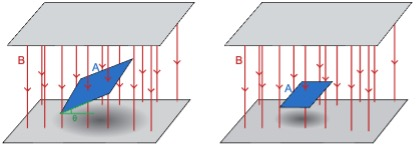
\includegraphics[width=5in]{fig1.jpg}
    \end{center}
    \renewcommand{\baselinestretch}{1}
    \small\normalsize
    \begin{quote}
    \caption[Magnetic Flux]{Magnetic Flux \cite{noauthor_what_nodate}.} \label{fig: f1}
    \end{quote}
\end{figure}

\subsection{Electromagnetic Induction}
Induction is the main principle on which WPT relies. Faraday’s law of electromagnetic induction says that changing 
magnetic flux can induce an electromotive force (EMF) in a circuit:
\begin{equation}
    \mathcal{E} = -\frac{d\Phi_B}{dt}
\end{equation}
For example, when a current flows through a coil of wire, it creates a magnetic field.  If another object such as 
the receiving coil of wire comes into close range with the magnetic field, a current is induced in it momentarily 
\cite{young_university_2016}. However, if the current in the receiving coil continues to change in time, so does 
the magnetic field, and this changing magnetic field is able to sustain an AC current in the receiving coil 
\cite{young_university_2016}. It can be said that the transmitting coil is inducing an AC current in the receiving coil.  

Nikola Tesla discovered that electromagnetic induction could be used to seemingly transfer power through the air 
in the late 1800s \cite{lu_wireless_2016}.  Simple radio antennas have functioned via this method 
of power transfer since Tesla’s time, but until recently, it has not been used in cars and other electronics 
like Tesla had originally hoped \cite{lumpkins_nikola_2014}.  This is because the efficiency of this charging method over 
long distances or for larger applications did not appear to be economical, but with recent research the efficiency 
has been proved to be higher than originally thought \cite{lu_wireless_2016}.  

\subsection{AC to DC Current Conversion}
In order to charge a battery, a DC current is necessary, but the induced current is an AC current. 
A circuit element called a diode is necessary to convert AC current into pulses of DC current. 
A diode is a device with two terminals that only allows current to flow in one direction \cite{young_university_2016}. 

A rectifier is a more sophisticated version of a diode that is necessary in complex circuitry like that of EVs. 
The simplest of rectifiers, a single-phase half-wave rectifier, allows only the positive part of a sinusoidal AC 
current to pass through and into the battery \cite{skvarenina_power_2001}.  Single-phase full-wave rectifiers are able to 
convert the positive part of the sinusoidal AC current and the inverted negative part of the sinusoidal AC current 
into DC current \cite{skvarenina_power_2001}.  As shown in Figure \ref{fig: f2}, it is far more complicated and requires the use of four 
diodes. 

\begin{figure}
    \begin{center}
    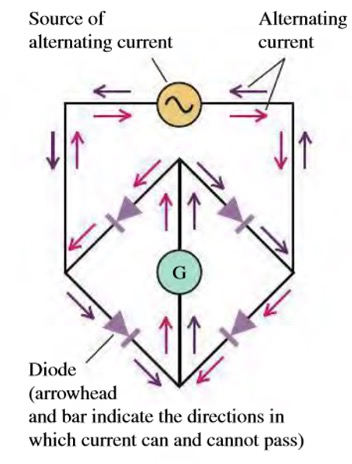
\includegraphics[width=3in]{fig2.jpg}
    \end{center}
    \renewcommand{\baselinestretch}{1}
    \small\normalsize
    \begin{quote}
    \caption[A DC current is established across the galvanometer]{A DC current is established across the galvanometer (represented by the G) \cite{young_university_2016}} \label{fig: f2}
    \end{quote}
\end{figure}

\subsection{Magnetic Resonance}
A transmitting coil (or circuit) can be designed so that its resonant frequency is the same as the frequency of 
the AC current in the transmitting circuit, inducing a current in the receiving circuit that has the greatest 
amplitude (meaning the greatest EMF) \cite{young_university_2016}. As shown in Figure \ref{fig: f3}, the amplitude greatly 
increases near the natural oscillating frequency. The natural oscillation frequency of the circuit can be manipulated 
by changing the strength of various circuit elements such as inductors, capacitors and resistors, or by changing the 
number of windings in the coil.  Alternatively, the current in the transmitting coil can be chosen based on a known 
natural oscillation frequency of the receiving circuit.

\begin{figure}
    \begin{center}
    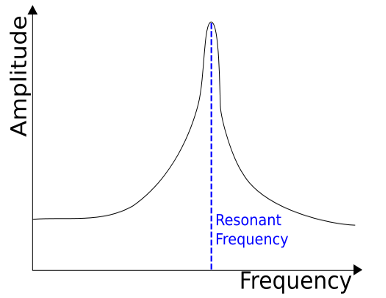
\includegraphics[width=3in]{fig3.png}
    \end{center}
    \renewcommand{\baselinestretch}{1}
    \small\normalsize
    \begin{quote}
    \caption[Voltage Amplitude vs. Frequency]{Voltage Amplitude vs. Frequency \cite{noauthor_resonant_nodate}.} \label{fig: f3}
    \end{quote}
\end{figure}

\section{Existing Methods}
\subsection{Wireless / DWPT Charging}
DWPT will allow EVs to drive further without having to stop to charge the battery for an extended period of time. 
Many companies are already researching ways of wirelessly charging batteries for devices. A thorough review of 
existing research was conducted prior to determining our research’s focus.

\subsection{Stationary Wireless Charging }
Stationary wireless charging is one method of charging currently being tested. Stationary charging is when the 
vehicle has a charging pad mounted on its underside and the driver parks overtop of the charging pad on the floor. 
This allows a signal to be picked up between the two pads and charges the vehicle 
\cite{fisher_electric_2014}. Energy is converted from AC to DC using a power converter which then 
transfers the energy back to the battery bank. The charging time of using stationary wireless charging depends on a 
variety of different variables including the source power level, charging pad sizes, and air-gap distance between 
the two windings \cite{panchal_review_2018}. These stationary wireless charging stations can also be installed 
in parking garages, homes, park ‘n’ ride facilities or even shopping centers. This type of wireless charging 
alleviates the hassle for the consumer because they do not have to worry about forgetting to plug in their car at 
night or dealing with trying to plug their car in if it is raining outside. This stationary charging technique is 
being applied to public transportation systems. For example, electric busses are trying this because they take an 
extended period of time to load and unload passengers at stops. They can gain some power to charge their batteries 
from these stationary pads at bus stops. This is known as “opportunity charging” \cite{lukic_cutting_2013}. 
This will allow electric city buses to cut down on their battery sizes and in turn their weight. Using this same 
technology could potentially reduce the size of heavy batteries in EVs. 

There have been numerous stationary wireless charging prototypes designed, each one with the location of the 
charging pad in different areas of the car such as the front, rear, and center of the car. Evatran is a company 
working on “Plugless Power” for passenger cars with the receiver pad location in the front of the car. With their 
prototype they can achieve an air gap distance of 102 mm with an efficiency of 90\% power transfer 
\cite{panchal_review_2018}. This company is just one of the many that are researching the stationary wireless 
power transfer, but overall, the prototypes have been developed with an air-gap distance of 100-300 mm with an 
efficiency from 71 to 95\% \cite{panchal_review_2018}. 

\subsection{Dynamic Wireless Power Transfer (DWPT)}
\label{sec: s2.4.3}
DWPT is when a vehicle is moving and picking up a charge simultaneously. This usually involves a charging pad with 
coils connected to the bottom of the vehicle and another set of charging pads with coils underneath the road that 
are each activated for a split second as the vehicle passes over it \cite{fisher_electric_2014}.  
This could potentially transfer power from a non-moving transmitter, like the pad underneath the road, to the 
receiver coil of a moving object, like the vehicle. Many issues arise with DWPT systems, like low power transfer 
efficiency, and the considerable power loss that occurs \cite{rakhymbay_precise_2018}. Currently, a University of Auckland 
research team has designed a prototype of a 400 m long stretch of track that wirelessly transmits 100 kW of power 
to a train \cite{rakhymbay_precise_2018}. Another team from the Oak Ridge National Laboratory has proven that the 
efficiency of the power transfer of a DWPT system depends on the position of the transmitter coil with respect to the 
pickup coil \cite{rakhymbay_precise_2018}. What this essentially means is that the position that a vehicle travels overtop 
of the coils in the road greatly impacts how much power can be drawn. To minimize this problem of power loss due to 
lateral misalignment there have been many methods proposed to maximize the lateral misalignment tolerance. These 
methods include changing the geometry of the coil, placing multiple coils in an orthogonal configuration, overlapping 
the configuration of the coils, or using different geometry of several different coils in one unit 
\cite{karam_hwang_autonomous_2017}. 

At this time, circular coils and Double D (DD) coils are the common type for the pad arrays. DD coils have a 
higher coupling coefficient and a higher offset tolerance \cite{xiang_design_2017}. This means 
that you get a higher fraction of magnetic flux produced by the DD coils compared to the circular coils. 
There is a new design of DD coils proposed that uses DD coils in a crossed design as shown in Figure \ref{fig: f4}. 
Unlike the original, the crossed DD design will offset the coils so that the edges are not flushed against each other. 
The results concluded that when the conventional DD coil is chosen as the primary pad type the average output of 
power was 7.1528 kW and the efficiency was 84.02\% and when the crossed DD was chosen the average output of power 
was 11.517 kW and the efficiency was 91.79\% \cite{xiang_design_2017}. The report concluded that 
26\% more energy can be transferred while using DWPT with this crossed DD design of the coils \cite{karam_hwang_autonomous_2017}. 

\begin{figure}
    \begin{center}
    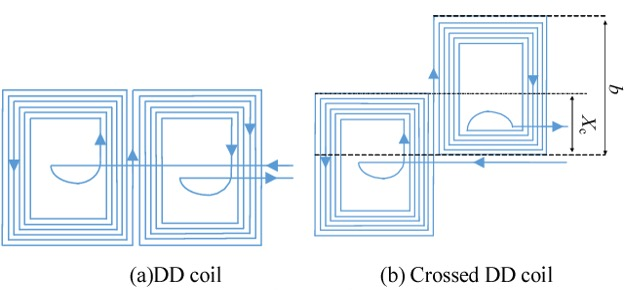
\includegraphics[width=5in]{fig4.jpg}
    \end{center}
    \renewcommand{\baselinestretch}{1}
    \small\normalsize
    \begin{quote}
    \caption[Difference between the alignment of DD coils and the crossed DD coils]{Difference between the alignment of DD coils and the crossed DD coils \cite{xiang_design_2017}.} \label{fig: f4}
    \end{quote}
\end{figure}

For maximum efficiency of power transfer in DWPT the vehicle has to be aligned on the road in the right orientation. 
Misalignment of the vehicle is inevitable since a person is physically driving and controlling the vehicle. 
A proposed method to change this is to use an autonomous coil alignment system for EVs that will detect misalignment 
and then the lateral position of the EV would be self-adjusted by an autonomous steering function 
\cite{karam_hwang_autonomous_2017}. 

\subsection{Magnetic Resonance Coupling}
Magnetic resonance coupling is another technique companies are using to wirelessly charge batteries. 
With this method there are two different resonators. One of the resonators receives energy from an 
external power supply while the other resonator is physically separated from the first and is used to 
supply working power to an external load \cite{ho_comparative_2011}. Both of these resonators are trying 
to oscillate at the same resonant frequency to produce the greatest amplitude. This transfers non-radiative 
energy between both resonators through coupling of the resonant-field evanescent tails \cite{ho_comparative_2011}. 
An evanescent field is an oscillating electric field in which the energy is spatially concentrated around the source, 
so this essentially takes the non-radiative energy and couples it with the oscillating electric field. Using a pair 
of rectangular spiral copper windings with the same shape and structure can help achieve efficient wireless energy 
transfer. With this system the receiver output voltage decreases linearly with an increase in the distance between 
the transmitter coil and the receiver coil \cite{ho_comparative_2011}. The main company that is researching this 
type of DWPT is Witricity. Using this method of magnetic resonant coupling, DWPT can have an efficiency of 90\% 
and a power transfer rate of up to 3.3 kW. What this essentially means is that the electromagnetic waves produced 
by the resonators can be used to transfer energy. To ensure that this works and that resonant objects can exchange 
energy efficiently, the correct resonant frequency has to be calculated. There are many benefits to using this 
technique to charge objects wirelessly. With magnetic resonance coupling you can get long transmission distance 
and no radiation, but it is difficult to adjust the resonant frequency if you are trying to charge multiple devices 
or objects \cite{parmesh_wireless_2017}. Magnetic resonance is currently being used to wirelessly charge phone 
batteries, but the research done on the different coil shapes, sizes, and their efficiency can still be used to guide 
our research on wirelessly charging EVs.

\section{Limitations}
\subsection{Safety}
The most significant safety limitation related to DWPT is electromagnetic field exposure. The medical community is 
somewhat split on categorizing the effects of electromagnetic field exposure as either beneficial or detrimental to 
human health. There are claims that applications of electromagnetic fields, even those generated from cellphones, 
have cognitive benefits \cite{arendash_electromagnetic_2010}. Other experts warn that electromagnetic field exposure could promote 
cancer and increase risk of miscarriage \cite{kostoff_combined_2013}. While the levels for which electromagnetic fields are 
considered beneficial or harmful are unestablished, the International Commission on Non-Ionizing Radiation Protection 
(ICNIRP) sets 6.25 µT as the acceptable limit for the public.  The Oak Ridge National Laboratory measured the 
electromagnetic field at 9 different positions above a wireless power transmitter coil and found that it peaked at 
about half the allowable limit for 8 of the 9 positions \cite{onar_novel_2013}. For the one position where the measured 
electromagnetic field was over 3 times the allowable, a strategically placed thin aluminum sheet brought it down to 
just under 6 µT \cite{onar_novel_2013}. While electromagnetic field exposure is a concern that can easily be remediated, 
the possible effects of an induced magnetic field on medical devices such as pacemakers may be harder to manage.

In simple terms, pacemakers are medical devices that help regulate the heartbeat, typically implanted after some 
heart-related emergency. Because they are electronic, they are susceptible to being adversely affected by magnetic 
fields. If a pacemaker were to act irregularly due to electromagnetic field exposure, it could cause significant 
health issues or even death for the user. A study published in the medical journal EP Europace examined the effects 
of electromagnetic fields on pacemakers and implantable cardioverter-defibrillators (ICDs). They found that even at 
levels of 300 µT, no noticeable or detrimental effects were detected on the implanted devices 
\cite{tiikkaja_electromagnetic_2013}. As mentioned before, in experimental trials of DWPT, the measured electromagnetic 
field remained at about 1\% of that used in the medical trial.

Electromagnetic field exposure is a safety concern that should be monitored but should not prevent the implementation 
of DWPT in public roads. The electromagnetic fields generated are not expected to exceed the safe limit for the public 
and will not pose a threat to those with implanted medical devices. Electromagnetic shielding – the use of a material 
to block an electromagnetic field – is possible, as demonstrated by the Oak Ridge lab in their DWPT trial. Graphene 
foam composites are most efficient for shielding, having a high shielding effectiveness and desirable material 
properties, such as being lightweight and flexible \cite{chen_lightweight_2013}. The implementation of electromagnetic 
shielding could increase the cost of constructing a DWPT road. When analyzing the economics of implementation, 
this is something that would need to be considered.

\subsection{Cost of Implementation}
The cost of full-scale implementation is generally calculated from a design perspective, as DWPT is still in testing 
and development. The factors that must be taken into consideration are the coils of an optimized size required to 
charge an EV, the cost of removing the road to install the coils, and the cost of repaving the road after installation 
\cite{chen_lightweight_2013}. Costs could be reduced by implementing DWPT into roads that are already in need of repaving. 
Furthermore, the energy required to keep such coils powered throughout the day must also be considered, making sure 
that peak hours are given extra energy to compensate for increased vehicular traffic \cite{chen_lightweight_2013}. 
The following analysis of cost will be qualitative, as not much research has been done on the quantitative cost. 

The length of individual coils must be calculated empirically. However, as mentioned previously, full scale 
implementation is still novel and companies who have obtained successful results are reluctant to share their 
findings. The total raw material cost would consist of the length required for each coil multiplied by the number 
of coils installed over the given length of road. Infrastructure costs will vary, depending on the chosen power supply. 
For solar power, the installation costs of solar panels must be taken into consideration. What must be determined is 
the number of coils that can be powered per solar panel \cite{chen_lightweight_2013}). If an alternative source of power is used, 
the cost of that power must be determined. 

Furthermore, a significant portion of the cost of implementation will be the physical installation of the coils. 
For initial implementation, one charging lane per highway would be sufficient, given the current usage rates of 
EVs \cite{li_longitudinal_2018}. Depending on the length of road used, the cost of removing the pavement and repaving the 
road after installation could outweigh the benefits of implementing wireless power transfer. As interstate 
highways are maintained by the state government, it is possible that some toll would be needed to fund a project 
of this magnitude. Still, some companies may not be convinced that the benefits of dynamic wireless power transfer 
outweigh the initial capital requirements \cite{chen_lightweight_2013}. 

Something that must be taken into consideration when implementing a DWPT lane on the roads is the change in traffic. 
Simulations have shown that having a DWPT lane can impact traffic in a negative manner \cite{li_longitudinal_2018}. EVs with 
lower battery charge will drive in the charging lane at a slower pace than other cars around them \cite{li_longitudinal_2018}. 
If a vehicle is going slow in a wireless charging lane, its battery will be more charged \cite{li_longitudinal_2018}. 
This is because the vehicle is spending more time in the charging lane and is not utilizing as much power. 
However, there are possible ways to alleviate this problem. One solution to this problem would be to require 
that cars be at a specific battery charge to be able to use the charging lane \cite{li_longitudinal_2018}. 
This will ensure that vehicles will not go slower in the charging lane. Additionally, there will be a significantly 
larger amount of traffic when actually constructing the lanes, which will take time to complete.

Another consideration when implementing a DWPT lane on the roads is the cost. The initial construction cost of 
implementing a DWPT lane would be about \$200/m or \$321,900/mi \cite{chen_lightweight_2013}. However, this is just an 
estimate and actual costs will vary. The expenses of road maintenance and providing the coils with power will be 
higher than a traditional road, which may require a toll on the DWPT lane similar to what we see on some HOV lanes 
on Interstates currently. There are many factors that need to be considered when implementing a DWPT lane. 
A charging station costs significantly less, but a DWPT lane is much more efficient, in terms of time, 
for an EV than charging stations. 

The design of the DWPT lane system will consist of several components. Two of the most important components are 
the transmitter and receiver coil \cite{throngnumchai_design_2013}. The transmitter coil will be on the road while 
the receiver coil will be on the EV (so that the vehicle will be able to receive the magnetic field emitted 
from the receiver coil). It is important that we shield the body of the EV from the magnetic field, so there 
will be material to differentiate the vehicle and receiver coil \cite{throngnumchai_design_2013}. Typically, asphalt 
concrete is used to construct roads. However, that material may damage the coil or reduce power transfer efficiency 
due to low permeability of the material. It is important to look at alternative concretes to make sure the transmitter 
coil stays intact. There are many variables to consider when designing a DWPT lane. Examples include different coil 
variables, how far apart the different coil circuits should be, what to put in the coil circuits to maximize power 
transfer, what road material to use, etc. \cite{panchal_review_2018}. The goal is to maximize power transfer 
efficiency and reduce cost.

\section{Conclusion}
EVs are the future of the transportation industry because they are a feasible solution to slow global warming by 
reducing CO2-equivalent emissions by 80\% \cite{helmers_electric_2012}. At present, the most significant limitation to 
EV use is the power system because of charging time and short range. If DWPT technology can be applied in the future, 
charging EVs will be much more convenient and require much less time. As a result, EVs will be a preferable option 
for drivers with all needs including long-distance travels.

The goal of our research has been to add to this volume of work by thoroughly studying the possible issues regarding 
safety, implementation, and other areas of DWPT for EVs. Our goal has been to find the optimized design of a system 
with maximization of electrical efficiency and cost-efficiency using DC power because research in use of DC power 
for this application is not as extensive. Developing a DWPT system using DC power with a high enough efficiency and 
low enough cost will enable EVs to become a feasible and attractive option for all drivers. 
%Chapter 3

\renewcommand{\thechapter}{3}

\chapter{Methodology}

\section{Introduction}
As previously stated, our team has attempted to answer our research questions by developing a mathematical model 
and evaluating its accuracy with a experimental model.  Our research questions are:

\begin{enumerate}
    \item[(1)]
    How can the dynamic charging of EVs be successfully implemented into a roadway?  
    \item[(2)]
    Would dynamic charging be able to provide enough power to a vehicle to make a difference in its overall range capability? 
    \item[(3)]
    Is dynamic charging a safe and reliable means of transmitting power to a vehicle in motion on the roadway, and would it affect a vehicle’s performance in other ways?   
    \item[(4)]
    Would a traditional roadway be able to accommodate dynamic charging, or would more nontraditional infrastructure need to be created?
\end{enumerate}

\section{Hypothesis}
By testing different values for the variables listed below, we can develop a recommendation to optimize the power 
output efficiency of a prototype of a dynamic wireless power transfer (DWPT) system for an electric vehicle (EV).
Variables:
\begin{itemize}
    \item Voltage of source [V]
    \item Wire gauge of transmitting coil []
    \item Number of turns in transmitting coil []
    \item Radius of transmitting coil [m]
    \item Wire gauge of receiving coil []
    \item Number of turns in receiving coil []
    \item Radius of receiving coil [m]
    \item Height of the receiving coil above the transmitting coil [m]
    \item Distance between closest edges of coils in road [m]
    \item Velocity of car [m/s]
    \item Material that encloses the transmitting and receiving coil []
    \item Alignment with coil []
\end{itemize}

Through our research we were able to develop a model that incorporates all of the variables except material and 
alignment of coil, although further research could be done to incorporate these variables.

\section{Simulations}
Our simulation is coded in MATLAB R2020a using basic characteristics of MATLAB and the Parallel Computing Toolbox 
in order to run simulations at a faster speed when possible. By starting with the verified and validated Biot 
Savart Magnetic Toolbox for MATLAB, a toolbox used for numerically calculating the magnetic field of filaments 
in a 3D field, a full DWPT simulation was able to be developed \cite{lqueval_lquevalbsmag_2020}. The simulations use two modified 
functions from the toolbox, BSmag\_add\_filament.m and BSmag\_get\_B.m and functions get\_field.m and get\_flux.m 
developed with some help from the toolbox, as well as a main.m which is responsible for running a batch 
(more than one) of scenarios. Each function is explained in detail below.

\subsection{General Approach}
The purpose of the simulations is to provide an estimate of the total charge a given configuration can provide 
to a car battery over a given distance, as well as the relative cost of that configuration to the persons building it.  
We don’t consider the costs of car owners to be a barrier to adoption, because the cost is negligible for each owner 
in comparison to the cost of the infrastructure. As previously explained in Section \ref{sec: s2.3}, the flux through 
a coil needs to be calculated in order to determine the induced current in the receiving coil. The first component 
of flux is magnetic field, so the field must be calculated for a 3D matrix of points surrounding the transmitting. 
This is the main purpose of the Biot Savart Toolbox. Once the field is plotted, the total flow through the imaginary 
“surface” created by the receiving coil must be calculated by adding up the field at each point of the receiving coil 
over its area. Finally, the induced emf can be calculated by numerically integrating the flux over time and the 
current can be determined using Ohm’s Law and the calculated resistance of the receiving coil. Since current is a 
flow of charge, the charge to the battery can be obtained by integrating the current over time.

While the concepts behind the simulation are simple, the computations quickly become unwieldy, 
which required much optimization of the simulation in order to prevent unnecessary repeated computations. 
This led to a segmented design where the configuration of the infrastructure, or the environment, is only 
calculated once for each unique configuration although there are many car configurations that can be “driven” 
through each. We made assumptions that edge effects are negligible compared to the effects of the nearby coils 
and ran the simulation for 1600 m (approximately 1 mile) for all scenarios. Both the numerical plotting of the 
magnetic field and the numerical integration of the flux through the car’s coil are hefty calculations which is 
why the Parallel Computing Toolbox is necessary to run a large batch of simulations. With 10 variables being 
considered, even trying 2 values for each value is not an insignificant task (210 = 1024). This required much 
discretion in terms of deciding which variables to spend time testing more rigorously. 

\subsection{BSmag\_add\_filament.m}
The function prototype is:
\begin{center}
function [BSmag] = BSmag\_add\_filament(BSmag, Gamma, I, dGamma)
\end{center}
The purpose of this function is to add a filament, 
in our case a coil, to the 3D space. It takes the following 
inputs and outputs to accomplish this shown in Table \ref{t1} and Table \ref{t2}:

\begin{table}[H]
    \caption[BSmag\_add\_filament.m Inputs]{BSmag\_add\_filament.m Inputs}
    \begin{center}
    \begin{tabular}{| p{0.2\textwidth} | p{0.1\textwidth} | p{0.6\textwidth} |}
    \hline
    Input & Units & Purpose \\
    \hline \hline
    BSmag & & The BSmag data structure that is at first empty but each time a filament is added, it holds the new number of filaments as well as the characteristics of each filament (Gamma, I, dGamma). \\
    Gamma & [m, m, m] & The filament point coordinates, in our case we translate a linearly spaced vector in radians to x, y, and z coordinates. \\
    I & [A] & The current through the coil, where the sign indicates the direction. \\
    dGamma & [m] & The filament max discretization step. \\
    \hline
    \end{tabular}
    \end{center}
    \label{t1}
\end{table}

\begin{table}[H]
    \caption[BSmag\_add\_filament.m Outputs]{BSmag\_add\_filament.m Outputs}
    \begin{center}
    \begin{tabular}{| p{0.2\textwidth} | p{0.1\textwidth} | p{0.6\textwidth} |}
    \hline
    Output & Units & Purpose \\
    \hline \hline
    BSmag & & The BSmag data structure updated to include the nth filament. This can be passed back into the function any number of times to add more filaments. \\
    \hline
    \end{tabular}
    \end{center}
    \label{t2}
\end{table}

Prior to calling this function it’s important to set the number of total filaments in the BSmag object to 0, 
so that it starts fresh for each scenario. In our simulations, we assume that the direction of current is 
alternating so each time a coil is added the sign of the current is reversed. As stated previously, 
this function was taken from the Biot Savart Toolbox, but unnecessary information was removed to improve 
performance \cite{lqueval_lquevalbsmag_2020}.

\subsection{BSmag\_get\_B.m}
The function prototype is:
\begin{center}
    function [X,Y,Z,BZ] = BSmag\_get\_B(BSmag, X, Y, Z, muRel)
\end{center}
The purpose of this function is to calculate the magnetic field 
for all points in the specified 3D space made up of X, Y, Z. It takes the following inputs and outputs to accomplish 
this as shown in Table \ref{t3} and Table \ref{t4}:

\begin{table}[H]
    \caption[BSmag\_get\_B.m Inputs]{BSmag\_get\_B.m Inputs}
    \begin{center}
    \begin{tabular}{| p{0.2\textwidth} | p{0.1\textwidth} | p{0.6\textwidth} |}
    \hline
    Input & Units & Purpose \\
    \hline \hline
    BSmag & & The BSmag data structure that includes information about the filaments. \\
    X & & Field points x-coordinate vector or matrix. \\
    Y & & Field points y-coordinate vector or matrix. \\
    Z & & Field points z-coordinate vector or matrix. \\
    muRel & & The relative permeability of the material. \\
    \hline
    \end{tabular}
    \end{center}
    \label{t3}
\end{table}

\begin{table}[H]
    \caption[BSmag\_get\_B.m Outputs]{BSmag\_get\_B.m Outputs}
    \begin{center}
    \begin{tabular}{| p{0.2\textwidth} | p{0.1\textwidth} | p{0.6\textwidth} |}
    \hline
    Output & Units & Purpose \\
    \hline \hline
    X & & Field points x-coordinate vector or matrix. \\
    Y & & Field points y-coordinate vector or matrix. \\
    Z & & Field points z-coordinate vector or matrix. \\
    BZ & [T] & The z-component of the magnetic field. \\
    \hline
    \end{tabular}
    \end{center}
    \label{t4}
\end{table}

The function takes a term muRel which we assume to be 1 in our simulations. The term was included in order to 
make it easier for future research to incorporate it by estimating the composite permeability of the material 
between the transmitting coils and the receiving coils. This could include asphalt or concrete that may obscure 
the coil in the road, air, and any components on the vehicle that may obscure the coils.  By setting muRel = 1, 
we assume vacuum permeability which is a limitation of our experiments. It’s a source of over overestimation 
of the results because the space between the coils is not actually as permeable as a vacuum, but since the space 
is made up of mostly air it is a fair assumption. As stated previously, this function was taken from the Biot 
Savart Toolbox, but unnecessary information was removed to improve performance \cite{lqueval_lquevalbsmag_2020}.  
This is why the function used in our simulations only returns the z-component of the field. We assume that the coils 
are aligned perfectly parallel to one another and the road, so the only component of the field that has an effect on 
the flux through the receiving coil is the perpendicular component, or the z-component. In reality they are not 
perfectly parallel and edge affects can have effects, so this is a limitation of our simulation and a source of error. 

\subsection{get\_field.m}
The function prototype is:
\begin{center}
    function data = get\_field(V, wireGauge, turns, radius, wireGauge\_car, turns\_car, radius\_car, height, original\_spacing, velocity, scenarioID, outputFolder)
\end{center}
The purpose of this function is to calculate the magnetic 
field and cost of the provided configuration and pass relevant information to get\_flux.m for each configuration 
of the car. It then returns a matrix of all of the inputs for each unique scenario, the cost, and the total charge 
calculated by get\_flux.m. It takes the following inputs and outputs to accomplish this as shown in 
Table \ref{t5} and Table \ref{t6}:

\begin{table}[H]
    \caption[get\_field.m Inputs]{get\_field.m Inputs}
    \begin{center}
    \begin{tabular}{| p{0.2\textwidth} | p{0.1\textwidth} | p{0.6\textwidth} |}
    \hline
    Input & Units & Purpose \\
    \hline \hline
    V & [V] & The voltage of the source. \\
    wireGauge & [] & The wire gauge of the transmitting coils. \\
    turns & [] & The number of turns of the transmitting coils. \\
    radius & [m] & The radius of the transmitting coils. \\
    wireGauge\_car & [] & The wire gauge of the receiving coil. \\
    turns\_car & [] & The number of turns of the receiving coil. \\
    radius\_car & [m] & The radius of the receiving coil. \\
    height & [m] & The vertical distance between the transmitting and receiving coils. \\
    original\_spacing & [m] & The distance between the closest parts of the transmitting coils. \\
    velocity & [m/s] & The velocity of the car. \\
    scenarioID & [] & The identifier for this unique 3D configuration of the environment. \\
    outputFolder & & The folder where any figures and data will be written. \\
    \hline
    \end{tabular}
    \end{center}
    \label{t5}
\end{table}

\begin{table}[H]
    \caption[get\_field.m Outputs]{get\_field.m Outputs}
    \begin{center}
    \begin{tabular}{| p{0.2\textwidth} | p{0.1\textwidth} | p{0.6\textwidth} |}
    \hline
    Output & Units & Purpose \\
    \hline \hline
    data & & The matrix that contains the unique inputs and outputs (total charge and cost) for each unique configuration of the receiving coil for the current configuration of the environment. \\
    \hline
    \end{tabular}
    \end{center}
    \label{t6}
\end{table}

The function also has a list of constants which are important for subsequent calculations shown in Table \ref{t7}.

\begin{table}[H]
    \caption[FORMULA Constants]{FORMULA Constants}
    \begin{center}
    \begin{tabular}{| p{0.2\textwidth} | p{0.15\textwidth} | p{.1\textwidth} | p{0.45\textwidth} |}
    \hline
    Input & Value & Units & Purpose \\
    \hline \hline
    increment & .1 & [m] & The resolution or the distance between the points in the 3D meshgrid. This needs to be one order of magnitude less than any inputs in order for best performance. \\
    muRel & 1 & [] & The relative permeability of the material. \\
    rho & .0171E-6 & [ohm-m] & The resistivity of copper. \\
    density & & [g/m3] & The density of copper. \\
    wireGauges & array & [] & An array of wire gauges needed all configurations. \\
    WireDiameters & array & [m] & n array of corresponding diameters to the wire gauge array. \\
    maxDistance & 1600 & [m] & The total distance traveled by the simulated car. In all simulations we used 1600 m or approximately 1 mile to determine the predicted charge per mile. \\
    dGamma & 1E9 & [m] & The filament max discretization step. \\
    filamentStep & 10 $\cdot$ radius & [1/m] & The number of points in each turn of the transmitting coils. Increase for better performance. \\
    tightness & 10000 & [1/m] & The tightness with which the coils are wrapped. Increasing tightness will make the coils wrapped more tightly, but we use a sufficiently large number so that it is as if the coils are wrapped perfectly tightly. \\
    \hline
    \end{tabular}
    \end{center}
    \label{t7}
\end{table}

This function does a series of numerical calculations to calculate the field in the specified 3D space. 
First, it determines coil characteristics from the wire gauges, which also allows the current to be 
calculated using V, resistance, and Ohm’s law. The cost is then calculated using the power (P = IV) 
and weight of wire. The cost also takes into account the cost of the copper wire and the cost of the 
solar panels that would be needed to power the design. In the next section, eight coils are placed on the 
3D space with alternating currents. In the next step the desired 3D matrix is plotted using linearly spaced 
vectors and then the field is calculated by calling BSmag\_get\_B. Next, the scenarios for the desired car 
configurations are determined and get\_flux.m is called for each of them. Finally, the data matrix returns 
the desired information for all of the car configurations for the current configuration of the environment.

\subsection{get\_flux.m}
The function prototype is:
\begin{center}
function totalCharge = get\_flux(turns, d\_car, turns\_car, radius\_car, height, spacing, velocity, rho, scenarioID, BZ, X\_M, Y\_M, increment, meshDistance, heightIndex, numberOfSquaresX, numberOfSquaresY, outputFolder).
\end{center}
The purpose of this function is to calculate the total charge over a specified distance for each configuration 
of the car and returns the value. This function can also be used to plot 3D renderings of the configuration 
and graph charge or current over time, but in the majority of cases this feature is not used because the 
final output is the only information of interest. It takes the following inputs and outputs to accomplish 
this as shown in Table \ref{t8} and Table \ref{t9}. The function also has a list of constants which are 
important for subsequent calculations as shown in Table \ref{t10}.

\begin{table}[H]
    \caption[get\_flux.m Inputs]{get\_flux.m Inputs}
    \begin{center}
    \begin{tabular}{| p{0.25\textwidth} | p{0.1\textwidth} | p{0.55\textwidth} |}
    \hline
    Input & Units & Purpose \\
    \hline \hline
    turns & [] & The number of turns of the transmitting coils. \\
    d\_car & [m] & The diameter of the wire of the receiving coils. \\
    turns\_car & [] & The number of turns of the receiving coil. \\
    radius\_car & [m] & The radius of the receiving coil. \\
    height & [m] & The vertical distance between the transmitting and receiving coils. \\
    spacing & [m] & The distance between the closest parts of the transmitting coils plus the diameter of the transmitting coils. \\
    velocity & [m/s] & The velocity of the car. \\
    rho & [ohm-m] & The resistivity of copper. \\
    scenarioID & [] & The identifier for this unique 3D configuration of the environment and car. \\
    BZ & [T] & The z-component of the magnetic field. \\
    X\_M	& & Field points x-coordinate vector or matrix. \\
    Y\_M	 & & Field points y-coordinate vector or matrix. \\
    increment & [m] & The resolution or the distance between the points in the 3D meshgrid. \\
    meshDistance & [m] & The distance required to calculate the field for all 7 coils. \\
    heightIndex & [] & The index of the node at the desired height in the z-direction. \\
    NumberOfSquaresX & [] & The number of nodes across the x-direction of the meshgrid. \\
    NumberOfSquaresY & [] & The number of nodes across the y-direction of the meshgrid. \\
    outputFolder & & The folder where any figures and data will be written. \\
    \hline
    \end{tabular}
    \end{center}
    \label{t8}
\end{table}

\begin{table}[H]
    \caption[get\_flux.m Outputs]{get\_flux.m Outputs}
    \begin{center}
    \begin{tabular}{| p{0.2\textwidth} | p{0.1\textwidth} | p{0.6\textwidth} |}
    \hline
    Ouput & Units & Purpose \\
    \hline \hline
    totalCharge & [C] & The total charge calculated over the specified distance for the unique configuration. \\
    \hline
    \end{tabular}
    \end{center}
    \label{t9}
\end{table}

\begin{table}[H]
    \caption[FORMULA Constants]{FORMULA Constants}
    \begin{center}
    \begin{tabular}{| p{0.25\textwidth} | p{0.125\textwidth} | p{.075\textwidth} | p{0.45\textwidth} |}
    \hline
    Input & Value & Units & Purpose \\
    \hline \hline
    distanceStep & increment & [m] & The resolution of the distance between each snapshot of the car traveling on the road. Set equal to increment for best results or multiply by some integer multiple for faster (but less accurate) results. \\
    efficiencyOfRectifier & 1 & [] & The efficiency of the rectifier. For our simulations we assume the current is perfectly rectified, although this is an implication and therefore a source of error. \\
    tightness\_car & 10000 & [1/m] & The tightness with which the receiving coils are wrapped. Increasing tightness will make the coils wrapped more tightly, but we use a sufficiently large number so that it is as if the coils are wrapped perfectly tightly. \\
    \hline
    \end{tabular}
    \end{center}
    \label{t10}
\end{table}

This function does a series of calculations to calculate the flux in through the coil as it travels through the 3D 
space. In order to run faster simulations, we use two of the central coils out of the 8 we plotted and then assume 
that through a large space the field is the same, and therefore the flux is the same. This was shown to be a fair 
assumption through tests comparing estimated values to actual values with no significant difference in the outputs. 
For each snapshot in time as the car travels down the road, the flux is calculated by filtering out irrelevant 
field locations and then integrating numerically using the trapz function over the x and y directions. 
Then the flux is copied and pasted to each of the corresponding locations in the array that represents the actual 
distance the car travels.  Using the flux array and corresponding time array, we are able to obtain the total 
charge accumulated in the battery over the desired distance, using numerical versions of the equations:
\begin{equation}
    \mathcal{E} = -N \frac{d\Phi}{dt}
\end{equation}
Where N is the number of turns in the receiving coil, $\Phi$ is the flux, t is the time, and $\mathcal{E}$ 
is the emf induced in the receiving coil. 
\begin{equation}
    I = \frac{\mathcal{E}}{R}
\end{equation}
Where R is the resistance of the coil in the car, and I is the current of the coil in the car.
\begin{equation}
    Q = \int{I dt}
\end{equation}
Where Q is the total charge stored in the battery. 

\subsection{main.m}
main.m function is responsible for calling get\_field.m for each unique 3D configuration of the variables and 
passing in desired values for the car configurations. This function utilizes the Parallel Computing Toolbox 
so that unique environmental configurations can be computed in parallel if multiple CPUs are needed and available. 
The data is written to a text file delimited by commas so that it can easily be imported into other programs for 
analysis. See Section \ref{sec: s4.1} for the values used for the variables and the results of the simulations.

\subsection{analysis.py}
A simple Python script was written in Python 3 in order to produce graphs that show the outputs of the simulations 
against each variable. This was used to determine which variables had the largest effects on the output and what 
configurations had the largest charge to cost ratio.  We know that with infinite resources it would be possible 
to complete this project, but without some idea of the cost to the government or entity completing the project 
the results wouldn’t be very valuable. 

Within the Python script, libraries pydrive \cite{nabel_pydrive_nodate}, google \cite{noauthor_breaking_nodate}, 
oauth2client \cite{noauthor_what_nodate} are used to import required data files. Data are processed as a data frame in 
the pandas library \cite{jeff_reback_pandas-devpandas_2021}, and matplotlib \cite{hunter_matplotlib_2007} is used 
to graph the outputs. For the first batch of data of smaller size, each entry of output data was iterated and compared 
with each other to analyze the target variable while having other variables being fixed. For the second batch of 
data of larger size, possible entries of each variable were iterated in order to fix required variables and analyzed 
target variables. See Section \ref{sec: s4.1} for detailed analysis and Appendix \ref{sec: appB} for code used in Batch 2.

\section{Experimental Model}
To validate the results of our simulations, we designed an experimental model. The experimental model uses a 
circular path to mimic a straight line. It consists of a wooden platform to place the transmitting coils on, 
a rotating metal shaft with another metal arm attached at the top, and a motor to rotate the shaft. 
We used a pulley system with a gear ratio of 1:9.33 to the motor and rotating shaft to control the speed of 
the rotation. The coils used were 1.75” in diameter. We placed 16 of these coils on the platform in a circular 
path and connected them to a power supply to generate an electromagnetic field over each of the coils. 
On the rotating arm, we attached a small wooden car using a threaded rod. The receiving coil was then 
attached to a wooden car using Velcro. As the arm rotated, the receiving coil would have a current induced 
onto it by interacting with the aforementioned electromagnetic field. We wired the receiving coil to a slip 
ring on the rod that would allow the wires to not be tangled as the rod rotated. The wires from the end of 
the slip ring were then connected to an oscilloscope to measure the resulting current that was induced onto 
the receiving coil. 

\subsection{General Approach}
Our goal with the experimental model is to determine how the simulations translate to a real-world scenario. 
We planned on running the model using different variable combinations to find the optimal real-world application 
of this technology; however, due to the COVID pandemic we had to fall back on our original goals. 
Our current goal is to prove that the technology is feasible by showing that there is an electrical 
output from the receiving coil. The experimental model is a proof of concept of the simulations, 
showing that the technology is feasible and could enable EVs to charge while driving.

\subsection{Construction of the Experimental Model}
\subsubsection{Pulley Subsystem}
 
\begin{figure}
    \begin{center}
    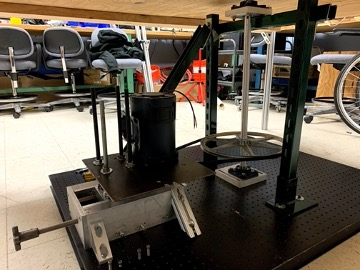
\includegraphics[width=5in]{fig5.jpg}
    \end{center}
    \renewcommand{\baselinestretch}{1}
    \small\normalsize
    \begin{quote}
    \caption[A picture showcasing the pulley subsystem]{A picture showcasing the pulley subsystem} \label{fig: f5}
    \end{quote}
\end{figure}

A 12V DC motor drives the vertical shaft of the rig via a v-belt pulley connection. The motor is mounted to 
a tensioner that maintains the proper belt tension. The tensioner is fixed to the optical breadboard. 
The speed of the motor is controlled by a variable DC power supply. Two ball bearings are used to constrain 
the vertical shaft. The bottom bearing is fixed to a plate that is secured in the optical breadboard. 
The top bearing is fixed to a plate that is supported by a green metal frame that is also connected 
to the optical breadboard. 

\subsubsection{Arm Subsystem}

\begin{figure}
    \begin{center}
    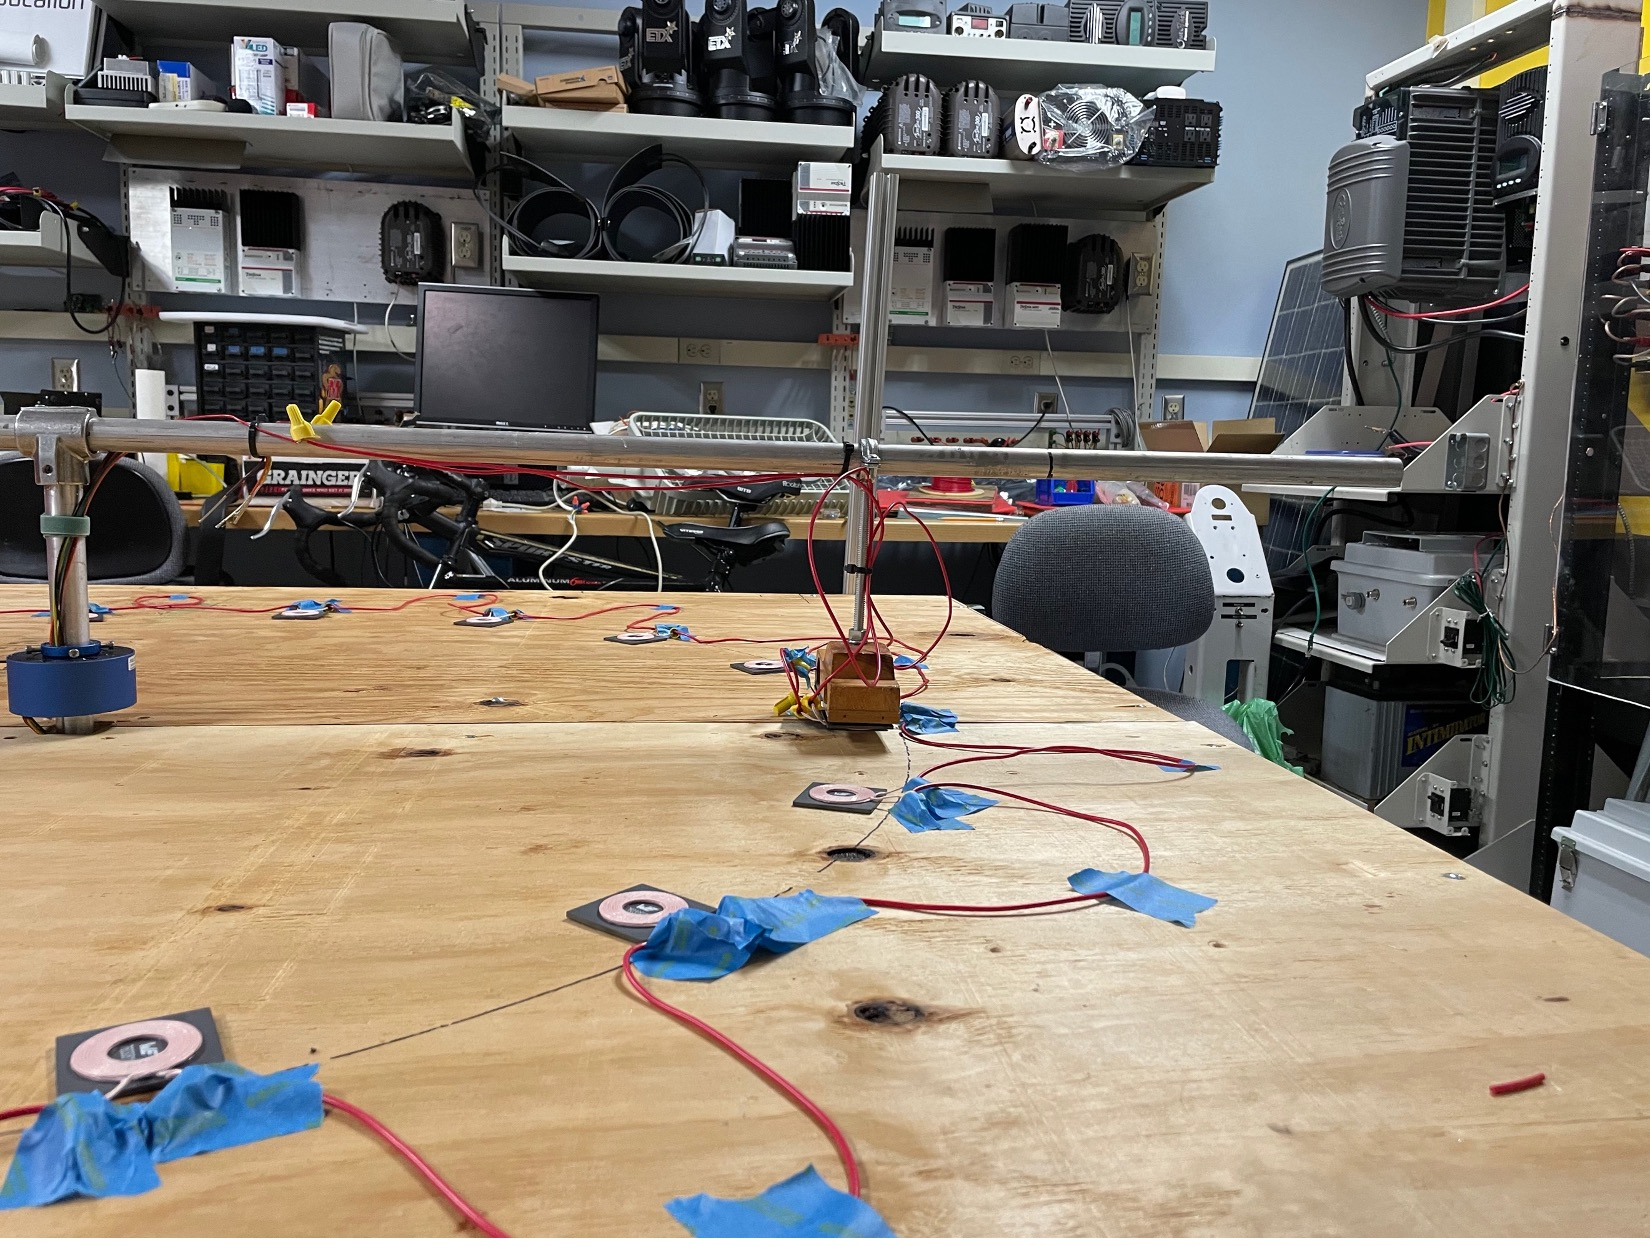
\includegraphics[width=5in]{fig6.jpg}
    \end{center}
    \renewcommand{\baselinestretch}{1}
    \small\normalsize
    \begin{quote}
    \caption[Rotating arm with vehicle attached]{Rotating arm with vehicle attached} \label{fig: f6}
    \end{quote}
\end{figure}

An aluminum T-connector connects the vertical shaft to the arm. This allows the arm to rotate at a 
constant angular velocity corresponding to the stepped down speed of the motor. The “vehicle” is 
mounted to the arm and travels in a circle to simulate DWPT. A slip ring is attached to the vertical 
shaft below the t connector. This prevents the wiring that travels along the arm from getting twisted 
as the rig rotates. 

\subsubsection{Transmitting Coils}

\begin{figure}
    \begin{center}
    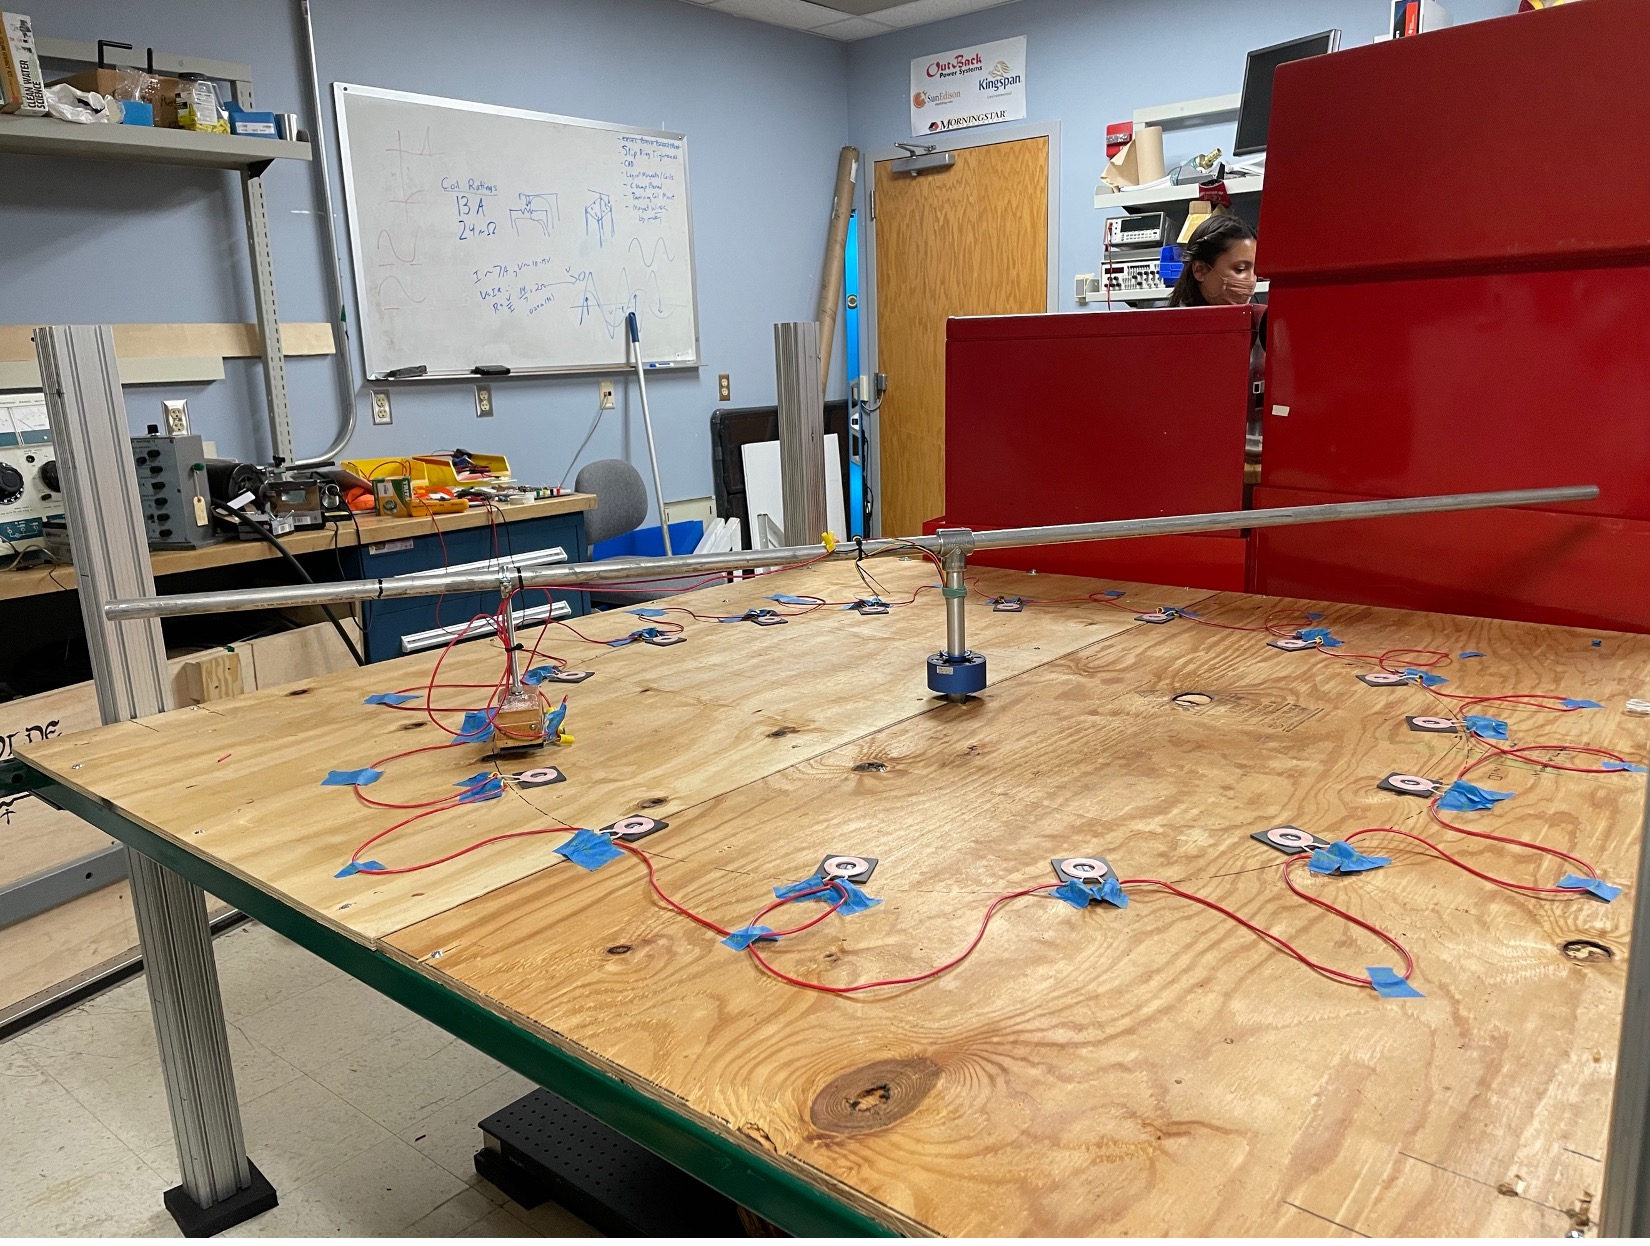
\includegraphics[width=5in]{fig7.jpg}
    \end{center}
    \renewcommand{\baselinestretch}{1}
    \small\normalsize
    \begin{quote}
    \caption[Transmitting coils laid out in a constant diameter]{Transmitting coils laid out in a constant diameter} \label{fig: f7}
    \end{quote}
\end{figure}

16 - 1.75” diameter coils are spaced evenly around a 2 ft diameter circle from the center of the experimental model. 
The coils are connected in series and powered through a variable DC power supply. Wire nuts are used to 
electrically insulate all connections. The total resistance of the coils is 0.3 $\Omega$ and the current 
rating is 11 A. These transmitting coils represent the coils that would be embedded in the road and transmit 
power to the passing electric vehicle.

\subsubsection{Receiving Coils}
 
\begin{figure}
    \begin{center}
    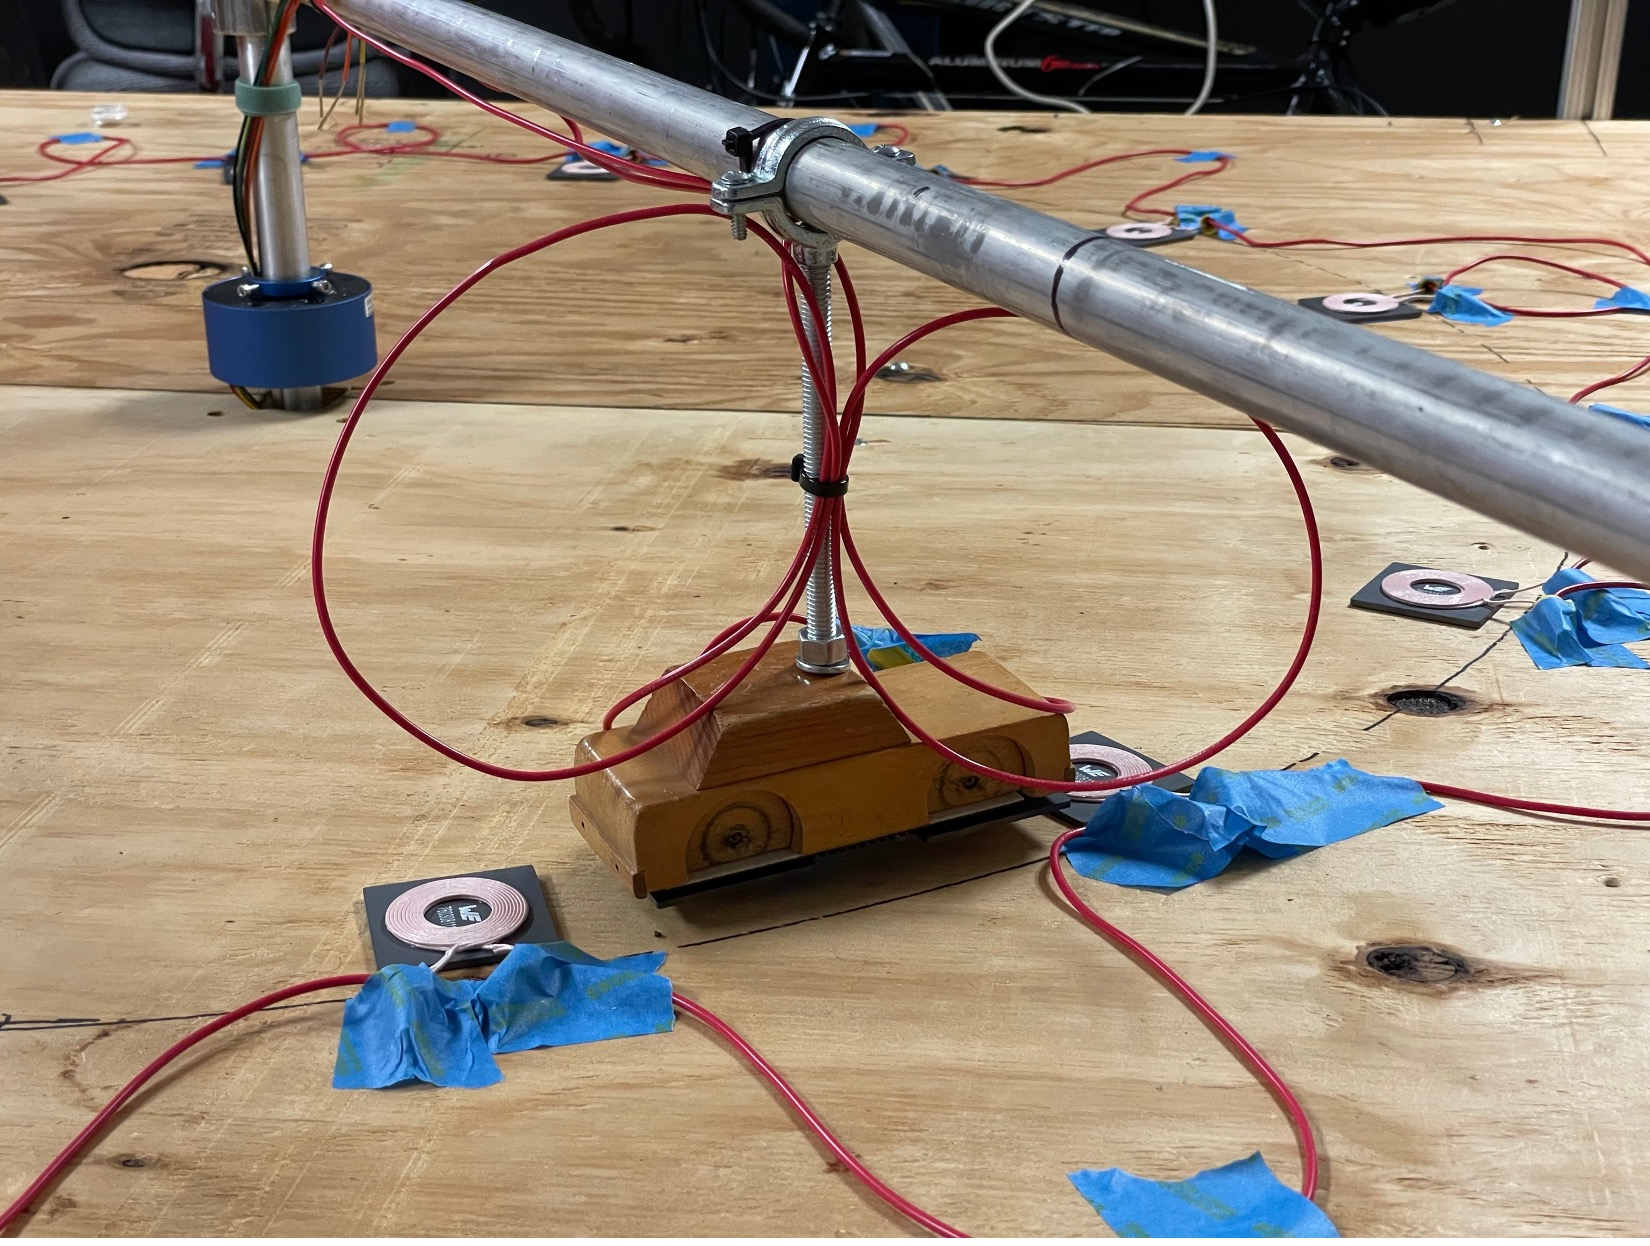
\includegraphics[width=5in]{fig8.jpg}
    \end{center}
    \renewcommand{\baselinestretch}{1}
    \small\normalsize
    \begin{quote}
    \caption[The wooden car with two transmitting coils attached]{The wooden car with two transmitting coils attached} \label{fig: f8}
    \end{quote}
\end{figure}

A wooden car is suspended from the spinning arm so that it travels over the transmitting coils. 
Two receiving coils are attached to the bottom of the wooden car to pick up the charge from the transmitting coils. 
These receiving coils are wired in series and the output is connected through the slip ring to an oscilloscope to 
gather data. The distance between the transmitting and receiving coils is less than ½ in.

\subsection{Operation of the Experimental model}
Preliminary cautions are taken into consideration prior to operation – care must be taken around voltage/current 
handling components, especially the power sources. Prior to working with the experimental model, operators must 
ensure that the deck is cleared of any obstacles or debris. A foot of distance, minimum, must be maintained 
between operators and the model while operational. When data collection is finished, operators must ensure 
that all electrical connections are detached from their respective power sources and turned off.

In order to initialize the rotational control, the power source must be connected to the motor controller. 
The frequency then has to be adjusted (from the controller) to match corresponding speeds required for data collection. 
Operators should be mindful to adjust frequencies gradually to avoid excess strain on the system. 
A tachometer is used to accurately measure the rotational speed.

For signal transmission, the output end of the transmitting coil is connected to an oscilloscope. 
Using an AC/DC signal (depending on stationary or rotational testing) via the waveform generator of the oscilloscope, 
the transmitting coil is powered. The transmitting coil is mounted to the rotating arm. 
From the oscilloscope, voltage and current are adjusted to suit the desired test data.

For recording data, a voltmeter or oscilloscope is attached to the receiving coils. 
While the experimental model is running, the induced EMF is measured and recorded on the receiving coils. 
Additionally, the relationships among the transmitting and receiving coils are recorded as well – specifically 
the turns ratio, frequency, vertical separation, and diameters.

\section{Limitations}

\subsection{Simulations}
Many assumptions made during the development will limit the applicability of the results to roads and 
decrease their accuracy, but these assumptions were necessary to make in order to construct a simulation 
that could be run in. a reasonable amount of time.

\subsubsection{Discretization}
All major computations done by the simulations are numerical in nature, meaning they are not exact since an 
exact solution is available for the multivariable integrations that are required in order to determine the 
field and flux at each point. Because the solutions are discretized, they are estimates of the actual values 
and there is more error the larger the step between each numerical calculation. Smaller steps require more 
time to calculate for the same space. Due to the large number of simulations necessary to obtain useful results, 
larger steps were used which introduced more error.  For the first and second bat h of simulations, 
the increment was set to .1 m due to time constraints, however, a preferred value is at least as small as 
.02 m because it produced < 1\% error when being used to calculate fluxes of coils in the range of our simulations. 
For our more specific recommendations, smaller steps could be used to obtain more accurate results. 
While the values may not be extremely accurate, what is important is that we have observed valuable 
trends in the data that can still help answer our research questions. 

\subsubsection{Vacuum Permeability}
In our simulations we assume vacuum permeability, as previously discussed. 
The space between the transmitting and receiving coils is not as permeable as a vacuum, 
so the flux through the receiving coil is actually smaller. Future research can incorporate 
this feature into the simulations by developing an equation for a composite material between the coils, 
but for the scope of our research this is a valid assumption because the space between the coils is mostly air.

\subsubsection{Tightness of Coils}
In the simulations we use a large value for the coils to simulate perfectly wrapped coils, but, 
coils will not be wrapped perfectly. They will likely be pancake coils. Our simulations are still applicable 
for pancake coils whose mean radius is equal to the radii used. As this is a common approximation used 
for pancake coils. Additionally, the simulation could be improved to map pancake coils instead of perfectly 
wrapped coils if desired. 

\subsubsection{Perpendicular Fields}
As previously discussed, we assume that only the z-component field contributes to the flux in the receiving coil, 
however this is not entirely accurate. Due to edge effects and small variations in the angle between the coils 
and the road surface, the coils will not be exactly parallel, so there are some effects of the x- and y-components. 
This is a reasonable assumption however, because even with small variations, the x- and y-component will 
be negligible compared to the z-component. 

\subsubsection{Uniform Fields}
A major assumption made in our simulations is that over a large distance the field variation will become uniform. 
During “start-up” and “shut-down” of the process experiences a greater change in flux, so the current at those 
locations would be greater. This is because you are transferring from a negligible field to a strong field or 
a strong field to negligible field, which is a bigger change than in the middle of the coils. 
This is a reasonable assumption based on preliminary tests run that showed that the difference is 
negligible compared to the overall change in flux.  As you can see in an example result from one of these tests 
in Figure \ref{fig: f9} to Figure \ref{fig: f12} the cumulative charge over time is very similar as well as the current over time, 
although you can see some small visible differences in the outputs. A large difference in the graphs would 
suggest that this assumption might not be valid or at least introduce significant error into our simulation, 
but it is clear that that is not the case. 

\begin{figure}
    \begin{center}
    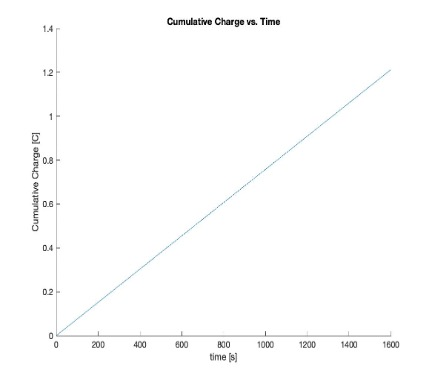
\includegraphics[width=3in]{fig9.jpg}
    \end{center}
    \renewcommand{\baselinestretch}{1}
    \small\normalsize
    \begin{quote}
    \caption[Cumulative Charge vs. Time (Not Estimated)]{Cumulative Charge vs. Time (Not Estimated)} \label{fig: f9}
    \end{quote}
\end{figure}

\begin{figure}
    \begin{center}
    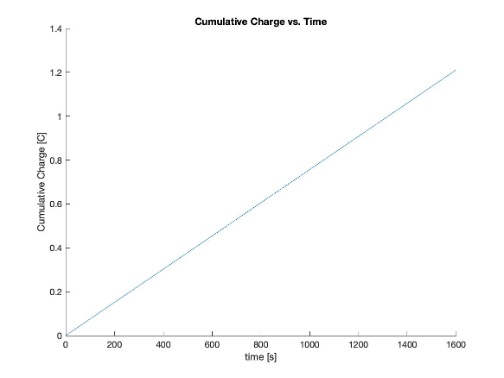
\includegraphics[width=3in]{fig10.jpg}
    \end{center}
    \renewcommand{\baselinestretch}{1}
    \small\normalsize
    \begin{quote}
    \caption[Cumulative Charge vs. Time (Estimated)]{Cumulative Charge vs. Time (Estimated)} \label{fig: f10}
    \end{quote}
\end{figure}

\begin{figure}
    \begin{center}
    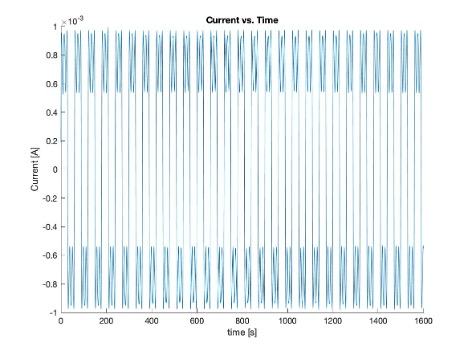
\includegraphics[width=3in]{fig11.jpg}
    \end{center}
    \renewcommand{\baselinestretch}{1}
    \small\normalsize
    \begin{quote}
    \caption[Current vs. Time (Not Estimated)]{Current vs. Time (Not Estimated)} \label{fig: f11}
    \end{quote}
\end{figure}

\begin{figure}
    \begin{center}
    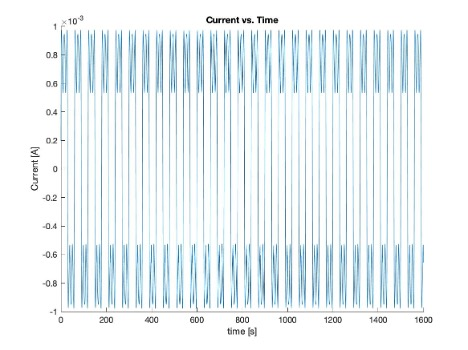
\includegraphics[width=3in]{fig12.jpg}
    \end{center}
    \renewcommand{\baselinestretch}{1}
    \small\normalsize
    \begin{quote}
    \caption[Current vs. Time (Estimated)]{Current vs. Time (Estimated)} \label{fig: f12}
    \end{quote}
\end{figure}

\subsubsection{Efficiency of the Rectifier}
In our simulations we assume that all the AC current induced in the receiving coil is converted to DC 
current without any losses. This is an overestimate, but it is a reasonable assumption because a quality 
rectifier would have negligible losses. This is also an area that can be improved on with further research.

\subsubsection{Perfect Alignment}
Our simulation assumes that the car coil can be perfectly centered above the transmitting coil at all times. 
It may be possible that drivers can remain in this position due to guides on the road and improvements in 
autonomous functions, or a mechanism like that mentioned in Section \ref{sec: s2.4.3} could be used. 
Another option would be to add a feature to the simulation to simulate poor alignment 
of the coils to determine how much of an effect misalignment has on charge output. 

\subsubsection{Constant Temperature}
Our simulation assumes a constant temperature of approximately $25^{\circ}C$. This is when the thermal 
expansion of all materials is neutral, and the resistances used in the simulation are valid. 
To address this assumption, future models will have to model resistance as function of temperature and 
consider the effects of thermal expansion and contraction of the materials in the road. 

\subsection{Experimental Model}

\subsubsection{Scalability}
The main assumption made about the applicability of the experimental model is scalability. 
The experimental model attempts to model a real-world highway on a smaller circular track. 
The alignment of the coils is not the same in a circular configuration as a highway one and 
trends observed at a smaller size might not scale very accurately to real world conditions. 
Further research will need to be done to model DWPT at more realistic highway conditions.

\subsubsection{Resources}
One other limitation we had in the construction of our experimental model was resources. 
As a Gemstone team, we had guaranteed funding of \$1800 and received an extra \$1000 from other sources. 
This limited us in terms of scope and the size of the model we could construct and test. 
Future research with more funding could build at a much bigger scale than we have. 
Additionally, an important resource we were lacking was time. This project was only ever going 
to last for four years as a Gemstone project, so we had to focus our scope again on what could 
realistically be accomplished in that timeframe. Additionally, the COVID-19 pandemic severely 
limited our amount of time in the lab with the transition to an online class structure. 
This affected our ability to gather as much data and test as many variables as we had hoped originally.

\subsubsection{Testing Variables}
There were multiple additional variables that we would have liked to have been able to test using 
our experimental model. The vertical separation between the transmitting and receiving coils was 
one of the most important ones. This was in our original plans for the model but we had to take it 
out due to the lack of time left in the project. Our original CAD model had a 3D printed part coming 
down from the arm that would have been able to be set at multiple different heights. We also wanted to 
test for the effect of an offset between the transmitting and receiving coils, where they are not perfectly 
in line with one another. Finally, one more variable we wanted to test for was the relationship between 
the sizes of the transmitting and receiving coils. To save time, we were only able to purchase one type of coil. 
This made it impossible to test for the differences between coil sizes on the receiving coil’s eventual output. 
%Chapter 4

\renewcommand{\thechapter}{4}

\chapter{Results}

\section{Simulations}
\label{sec: s4.1}
Determining results for the simulations was an iterative process. The first batch of simulations helped us to 
determine which variables did not influence the results and which had more effects. During the second batch we were 
able to test more scenarios to obtain more useful data by comparing charge output to cost. Analysis of the second 
batch allowed us to run a third smaller batch of simulations to obtain more accurate results for our final 
recommendations.

\subsection{Batch 1}
\subsubsection{Inputs}
For the of simulations the minimum and maximum predicted values for each variable based on the Society of Automotive 
Engineering Standard J2954 \cite{noauthor_j2954_nodate}. The voltage coming from the road was chosen based on the minimum and 
maximum voltages that solar panels come in, which is 96 and 100 volts respectively.  For the wire gauge, only 
standard wire gauge sizes were used since they come in standard sizes. The number of turns in the road coils, 
the number of turns was determined based on the amount in a pancake coil which is anywhere between 413 and 566 turns. 
The radius of the road coils was taken to be between 2.7 m and 3.7 m since this is the average width of low volume 
road width and standard lane width. 

The inputs for the coils that will be in the car is different since they will be the receiving coils. 
The wire gauge will still be the standard size for wire gauges, but the number of turns will be 229 for the 
minimum and 321 for the maximum. The radius for the coils will be 1.5 m for the maximum and 2.1 for the minimum 
and this comes from the average width of a compact car versus the average width of a full-size SUV since this 
will be the ranges of cars that will be on the road. 

The orientation of the coils in the simulation was also determined from research. For the height of the coils 
above the ground, the range of 0 to 0.5 m was chosen since the average vehicle ground clearance is 0.25 m. 
The Society of Automotive Engineers states that the most efficient spacing of coils would be no more than 18 cm 
between the closest parts \cite{noauthor_j2954_nodate}. Using this would mean that the spacing input for the simulation would 
be two times the radius of the coil for the minimum and two times the radius of the coil plus 0.3 m for the maximum. 
The velocity that is inputted into the simulation was 18 m/s for the minimum and 36 m/s for the maximum since this 
is the low highway speed to high highway speed. 

\begin{itemize}
    \item V = [96 600] [V]
    \item wireGauge = [8] []
    \item turns = [410 570] []
    \item radius = [2.5 4] [m]
    \item wireGauge\_car = [12] []
    \item turns\_car = [230 320] []
    \item radius\_car = [1.5 2] [m]
    \item height = [0 .5] [m]
    \item spacing = [0 .36] [m]
    \item velocity = [18 36] [m/s]
\end{itemize}

\subsubsection{Outputs}
The outputs of our simulation were compiled into graphs using analysis.py. Each graph shows the charge graphed 
against each variable. Outputs with the same inputs besides the varied value are connected by lines in order to 
show how a nearly identical simulation is affected by changing that variable. The first batch of simulations 
showed that velocity is not a factor in charge, which makes sense since the field is the same, see Figure \ref{fig: f20}. 
Figure \ref{fig: f13} shows the output charge versus voltage when the first simulation was run. This graph shows that as the 
voltage increases the output charge increases linearly. Figure \ref{fig: f14} shows the output charge versus the number of turns. 
As the number of turns increase the output charge decreases slowly. This shows that increasing the number of turns 
does not optimize the charge gained. Figure \ref{fig: f15} shows that output charge is only slightly dependent on the radius of 
the coil in the road since the slope is only increasing slightly. 
 	 
\begin{figure}
    \begin{center}
    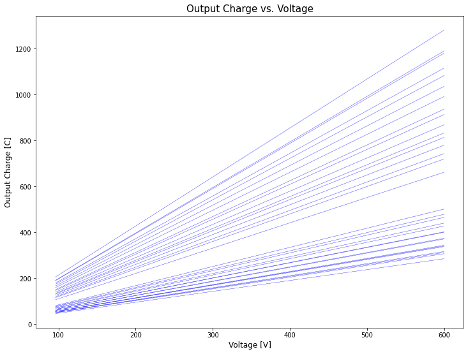
\includegraphics[width=3in]{fig13.png}
    \end{center}
    \renewcommand{\baselinestretch}{1}
    \small\normalsize
    \begin{quote}
    \caption[Batch 1 Output Charge vs. Voltage]{Batch 1 Output Charge vs. Voltage} \label{fig: f13}
    \end{quote}
\end{figure}

\begin{figure}
    \begin{center}
    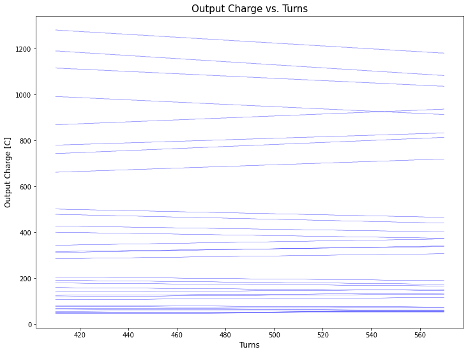
\includegraphics[width=3in]{fig14.png}
    \end{center}
    \renewcommand{\baselinestretch}{1}
    \small\normalsize
    \begin{quote}
    \caption[Batch 1 Output Charge vs. Turns]{Batch 1 Output Charge vs. Turns} \label{fig: f14}
    \end{quote}
\end{figure}

\begin{figure}
    \begin{center}
    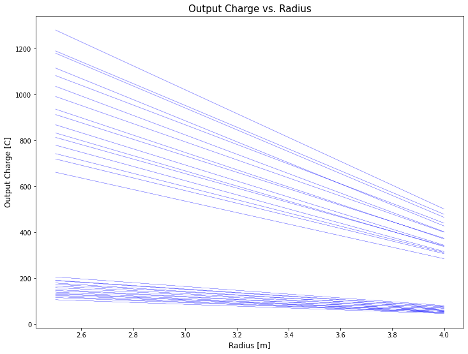
\includegraphics[width=3in]{fig15.png}
    \end{center}
    \renewcommand{\baselinestretch}{1}
    \small\normalsize
    \begin{quote}
    \caption[Batch 1 Output Charge vs. Radius]{Batch 1 Output Charge vs. Radius} \label{fig: f15}
    \end{quote}
\end{figure}

\begin{figure}
    \begin{center}
    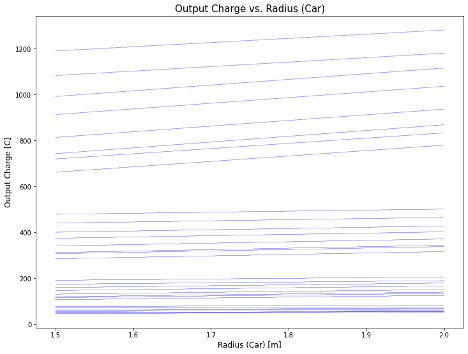
\includegraphics[width=3in]{fig16.png}
    \end{center}
    \renewcommand{\baselinestretch}{1}
    \small\normalsize
    \begin{quote}
    \caption[Batch 1 Output Charge vs. Radius of Coil on Car]{Batch 1 Output Charge vs. Radius of Coil on Car} \label{fig: f16}
    \end{quote}
\end{figure}

As for the coils in the car, Figure \ref{fig: f16} shows that the car coils radius has a bigger effect than the road coils 
radius on the output velocity. As the coils in the car start getting a bigger radius, the output charge decreases, 
so the coils in the car want to have a radius on the smaller side to optimize output charge. 
Figure \ref{fig: f17} shows that the number turns in the coil of the car increases the output charge. 
Figure \ref{fig: f18} shows that the height decreases the output charge goes down. As expected, as the spacing in the road 
increases, the output charge decreases as shown in Figure \ref{fig: f19}. 

\begin{figure}
    \begin{center}
    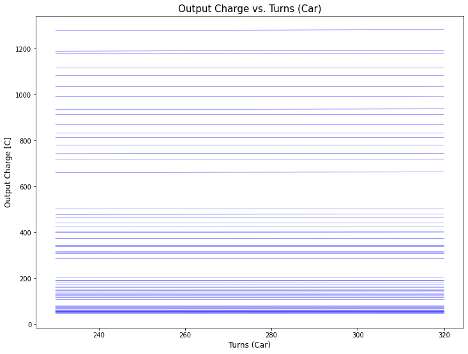
\includegraphics[width=3in]{fig17.png}
    \end{center}
    \renewcommand{\baselinestretch}{1}
    \small\normalsize
    \begin{quote}
    \caption[Batch 1 Output Charge vs. Turns of Coil on Car	]{Batch 1 Output Charge vs. Turns of Coil on Car} \label{fig: f17}
    \end{quote}
\end{figure}

\begin{figure}
    \begin{center}
    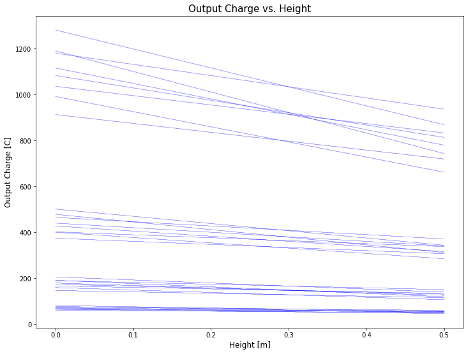
\includegraphics[width=3in]{fig18.png}
    \end{center}
    \renewcommand{\baselinestretch}{1}
    \small\normalsize
    \begin{quote}
    \caption[Batch 1 Output Charge vs. Height]{Batch 1 Output Charge vs. Height } \label{fig: f18}
    \end{quote}
\end{figure}

\begin{figure}
    \begin{center}
    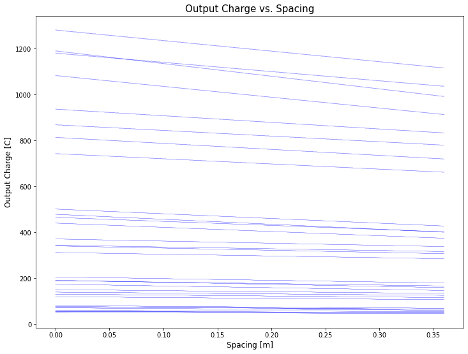
\includegraphics[width=3in]{fig19.png}
    \end{center}
    \renewcommand{\baselinestretch}{1}
    \small\normalsize
    \begin{quote}
    \caption[Batch 1 Output Charge vs. Spacing of Coils on Road]{Batch 1 Output Charge vs. Spacing of Coils on Road} \label{fig: f19}
    \end{quote}
\end{figure}

\begin{figure}
    \begin{center}
    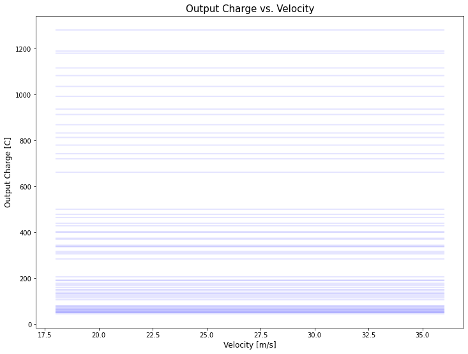
\includegraphics[width=3in]{fig20.png}
    \end{center}
    \renewcommand{\baselinestretch}{1}
    \small\normalsize
    \begin{quote}
    \caption[Batch 1 Output Charge vs. Velocity]{Batch 1 Output Charge vs. Velocity} \label{fig: f20}
    \end{quote}
\end{figure}

\subsection{Batch 2}
\subsubsection{Inputs}
Based on the outputs from Batch 1 the inputs were updated for a more refined set of simulations. 
We added a second option for both wire gauges in order to determine trends in those variables. 
In voltage, turns, radius, car turns, and car radius we added more values in the same ranges. 
For velocity we used 30 m/s because we found that velocity does not influence the charge output over the same 
distance. For height and spacing we replaced values with more realistic values of height and spacing in the original 
range. Below are the inputs for Batch 2, resulting in over 24,000 data points.

\begin{itemize}
    \item V = [100 250 450 600] [V]
    \item wireGauge = [6 8] []
    \item turns = [410 460 510 560] []
    \item radius = [1 2 3 4] [m]
    \item wireGauge\_car = [8 12] []
    \item turns\_car = [230 260 290 320] []
    \item radius\_car = [1.5 1.7 1.9 2.1] [m]
    \item height = [.15 .3] [m]
    \item spacing = [0 .18 .36] [m]
    \item velocity = [30] [m/s]
\end{itemize}

\subsubsection{Outputs}
Because Batch 2 has many more data points, we were able to observe more about the trends in the outputs. 
One important observation is that some variables do not impact cost of infrastructure, so optimal values 
for these can be as large as is reasonable for the physical configuration. These include wire gauge of the car 
coil, turns of the car coil, radius of the car coil, and height. Therefore, for Batch 3 we used only the values 
for these variables that correspond to the largest charge outputs. Other variables are worth looking into further. 
Voltage has a direct relationship with cost so for Batch 3 we used the value with the smallest corresponding 
cost/charge output, which is 100 V. Wire gauge has a constant relationship with cost, so we chose the largest 
charge value, which corresponds to 6-gauge wire.  Turns showed an interesting charge output so for Batch 3 we 
retested all values. Radius has a direct relationship with charge, however it experiences a huge drop off in output 
as radius increases, so it is worth a larger cost. Therefore, for Batch 3 we used only 1 m radius coils. 
For spacing, the trend is not increasing or decreasing for the entire time. For Batch 3, we tried more inputs 
in order to determine a better idea of the charge and cost correlations. We didn’y test spacing at 0 m because 
it clearly did not give a good charge output. See graphs below for each variable, excluding velocity as explained 
previously, for output charge, cost, and cost/charge. The graphs in Batch 2 (Figures \ref{fig: f21} through \ref{fig: f29}) are made in the same way as Batch 1, 
but there are additional graphs that graph cost vs. each variable as well as cost/charge vs. each variable.

\begin{figure}
    \begin{center}
    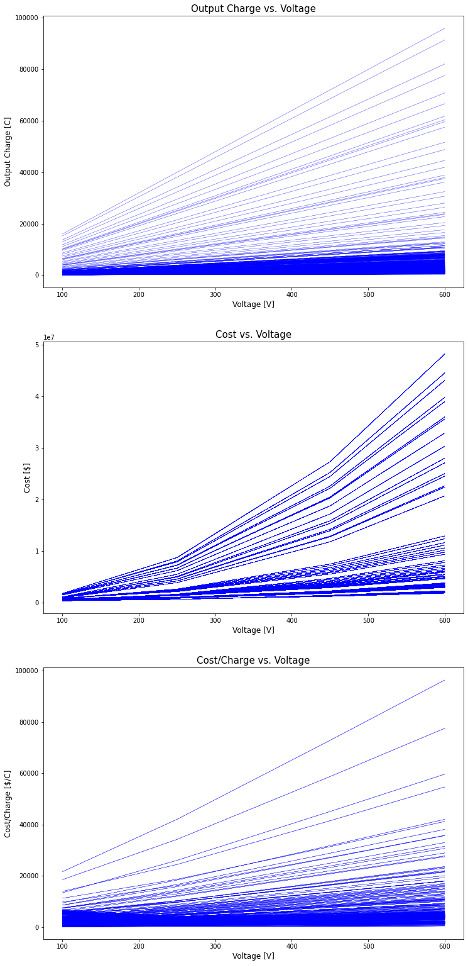
\includegraphics[width=3in]{fig21.png}
    \end{center}
    \renewcommand{\baselinestretch}{1}
    \small\normalsize
    \begin{quote}
    \caption[Batch 2 Voltage Trends]{Batch 2 Voltage Trends} \label{fig: f21}
    \end{quote}
\end{figure}

\begin{figure}
    \begin{center}
    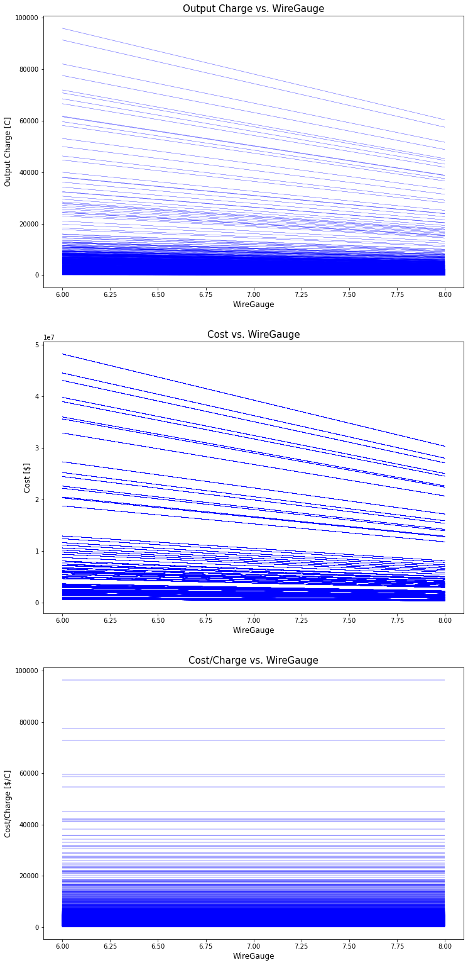
\includegraphics[width=3in]{fig22.png}
    \end{center}
    \renewcommand{\baselinestretch}{1}
    \small\normalsize
    \begin{quote}
    \caption[Batch 2 WireGauge Trends]{Batch 2 WireGauge Trends} \label{fig: f22}
    \end{quote}
\end{figure}

\begin{figure}
    \begin{center}
    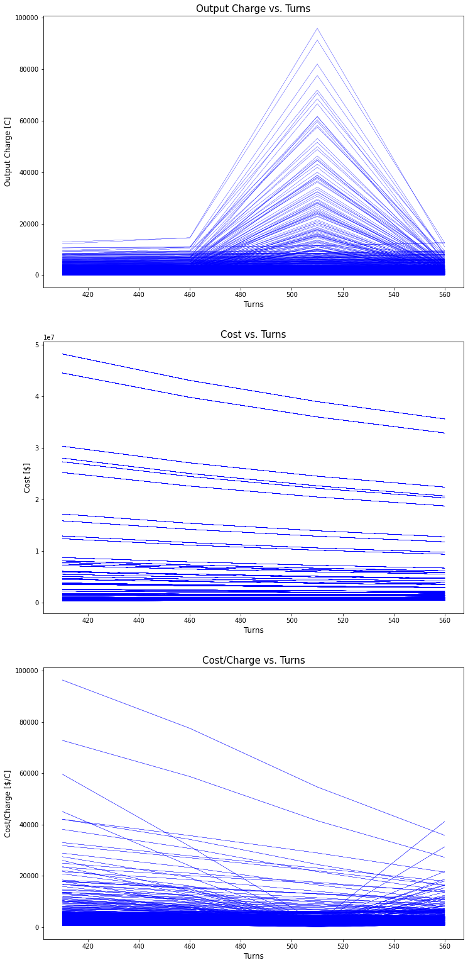
\includegraphics[width=3in]{fig23.png}
    \end{center}
    \renewcommand{\baselinestretch}{1}
    \small\normalsize
    \begin{quote}
    \caption[Batch 2 Turns Trends]{Batch 2 Turns Trends} \label{fig: f23}
    \end{quote}
\end{figure}

\begin{figure}
    \begin{center}
    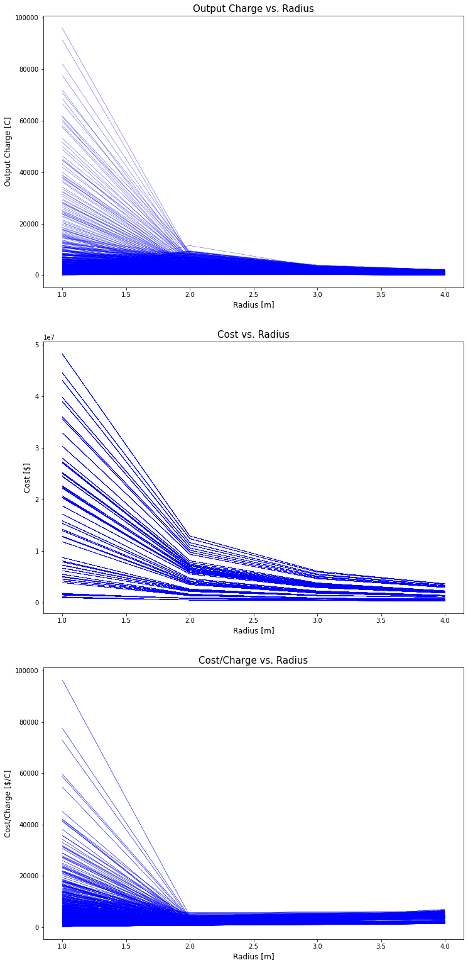
\includegraphics[width=3in]{fig24.png}
    \end{center}
    \renewcommand{\baselinestretch}{1}
    \small\normalsize
    \begin{quote}
    \caption[Batch 2 Radius Trends]{Batch 2 Radius Trends} \label{fig: f24}
    \end{quote}
\end{figure}

\begin{figure}
    \begin{center}
    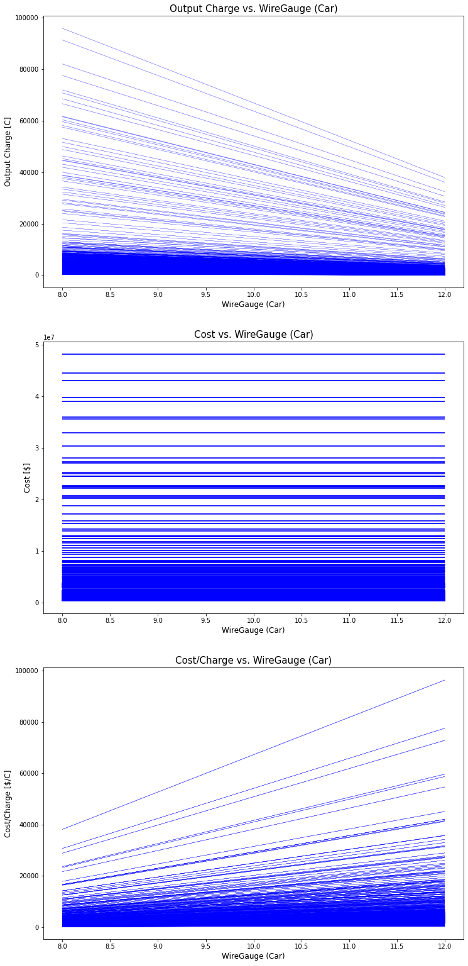
\includegraphics[width=3in]{fig25.png}
    \end{center}
    \renewcommand{\baselinestretch}{1}
    \small\normalsize
    \begin{quote}
    \caption[Batch 2 WireGauge (Car) Trends	]{Batch 2 WireGauge (Car) Trends	} \label{fig: f25}
    \end{quote}
\end{figure}

\begin{figure}
    \begin{center}
    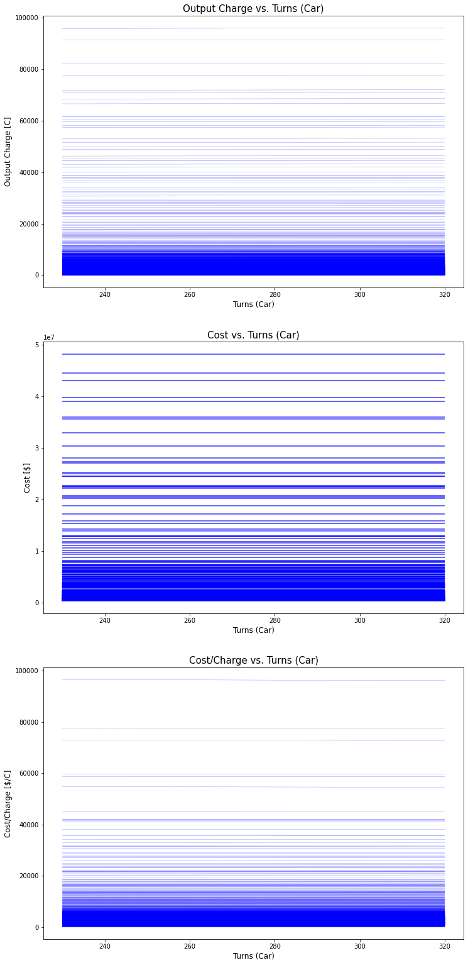
\includegraphics[width=3in]{fig26.png}
    \end{center}
    \renewcommand{\baselinestretch}{1}
    \small\normalsize
    \begin{quote}
    \caption[Batch 2 Turns (Car) Trends]{Batch 2 Turns (Car) Trends} \label{fig: f26}
    \end{quote}
\end{figure}

\begin{figure}
    \begin{center}
    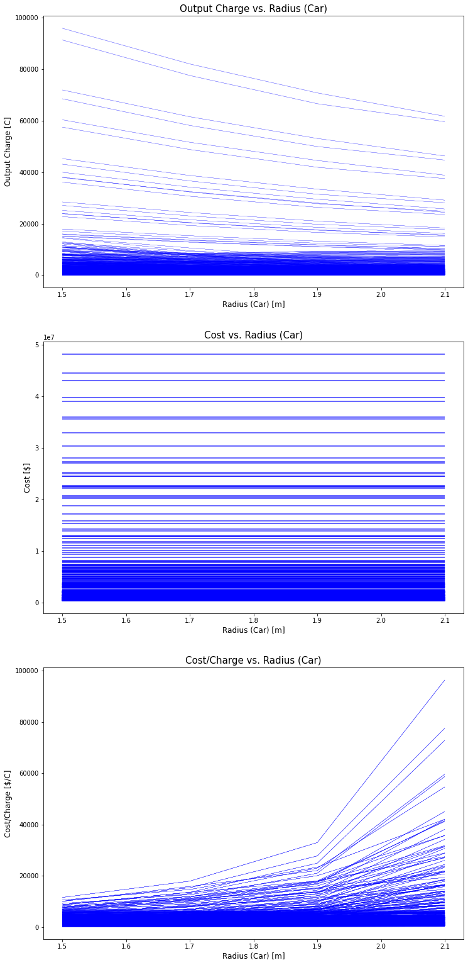
\includegraphics[width=3in]{fig27.png}
    \end{center}
    \renewcommand{\baselinestretch}{1}
    \small\normalsize
    \begin{quote}
    \caption[Batch 2 Radius (Car) Trends]{Batch 2 Radius (Car) Trends} \label{fig: f27}
    \end{quote}
\end{figure}

\begin{figure}
    \begin{center}
    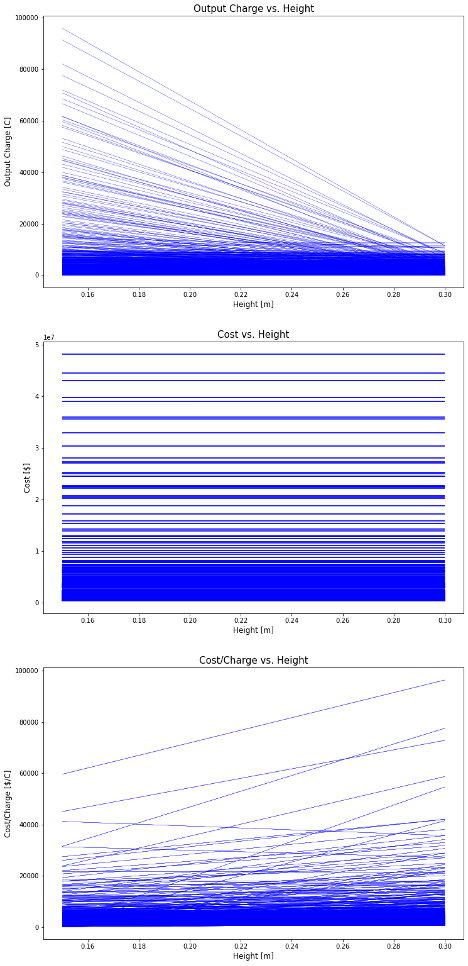
\includegraphics[width=3in]{fig28.png}
    \end{center}
    \renewcommand{\baselinestretch}{1}
    \small\normalsize
    \begin{quote}
    \caption[Batch 2 Height Trends]{Batch 2 Height Trends} \label{fig: f28}
    \end{quote}
\end{figure}

\begin{figure}
    \begin{center}
    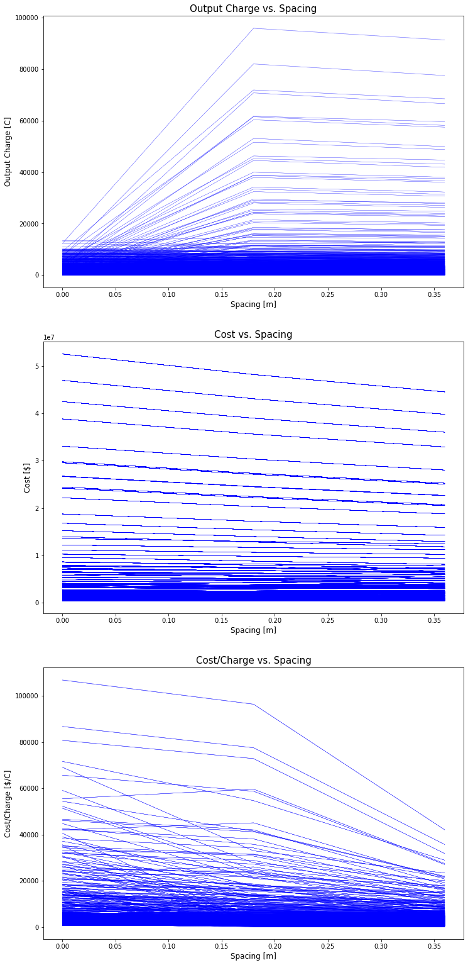
\includegraphics[width=3in]{fig29.png}
    \end{center}
    \renewcommand{\baselinestretch}{1}
    \small\normalsize
    \begin{quote}
    \caption[Batch 2 Spacing Trends]{Batch 2 Spacing Trends} \label{fig: f29}
    \end{quote}
\end{figure}

\subsection{Batch 3}
\label{sec: s4.1.3}
\subsubsection{Inputs}
The purpose of Batch 3 was to obtain more accurate values for charge. This is possible using smaller values of 
the increment (and therefore distanceStep) and filamentStep. We decreased the increment by a factor of 2 and 
increased the filament step by a factor of 10. This makes the mesh grid much finer, so many more calculations 
need to be done, which takes much longer. Therefore, we ran only 17 scenarios. We ran 16 scenarios to obtain 
more accurate values for economical configurations as determined from Batch 2 outputs. The inputs for the 
scenarios are below. 

\begin{itemize}
    \item V = [100] [V]
    \item wireGauge = [6] []
    \item turns = [410 460 510 560] []
    \item radius = [1] [m]
    \item wireGauge\_car = [8] []
    \item turns\_car = [320] []
    \item radius\_car = [1.5] [m]
    \item height = [.15] [m]
    \item spacing = [.09 .18 .27 .36] [m]
    \item velocity = [30] [m/s]
\end{itemize}

We ran one additional scenario that produced the largest overall charge in Batch 2. In case there is not an 
economical configuration that produces a reasonable charge output, it would be valuable to determine if any 
configuration would produce a reasonable charge output. The input for this scenario is below. 

\begin{itemize}
    \item V = [600] [V]
    \item wireGauge = [6] []
    \item turns = [510] []
    \item radius = [1] [m]
    \item wireGauge\_car = [8] []
    \item turns\_car = [320] []
    \item radius\_car = [1.5] [m]
    \item height = [.15] [m]
    \item spacing = [.09] [m]
    \item velocity = [30] [m/s]
\end{itemize}

\subsubsection{Outputs}
From analysis of the Batch 3 results, we can see that cost effectiveness decreases as both turns and spacing 
increase, so the most economical scenario corresponds to 410 turns and .09 spacing. This configuration output 
2142.7 C for 1600 m. See the Figures \ref{fig: f30} and \ref{fig: f31} below for the data trends.

\begin{figure}
    \begin{center}
    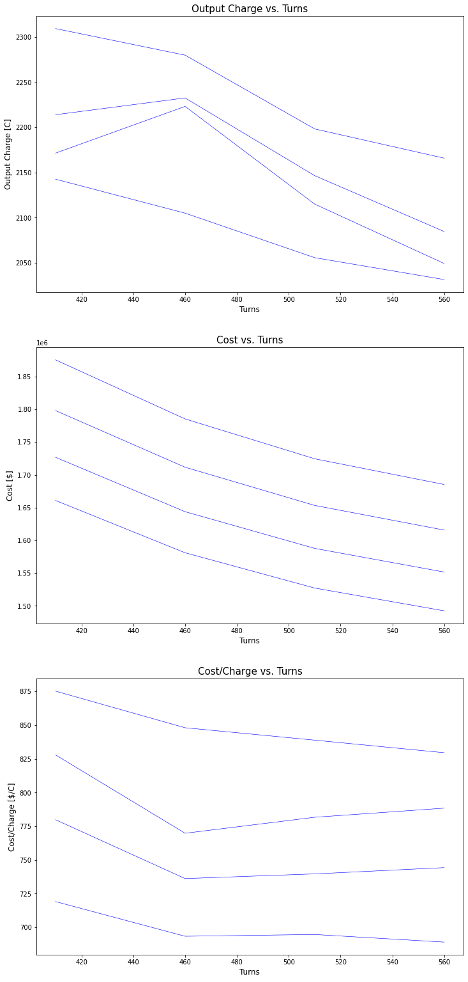
\includegraphics[width=3in]{fig30.png}
    \end{center}
    \renewcommand{\baselinestretch}{1}
    \small\normalsize
    \begin{quote}
    \caption[Batch 3 Turns Trends]{Batch 3 Turns Trends} \label{fig: f30}
    \end{quote}
\end{figure}

\begin{figure}
    \begin{center}
    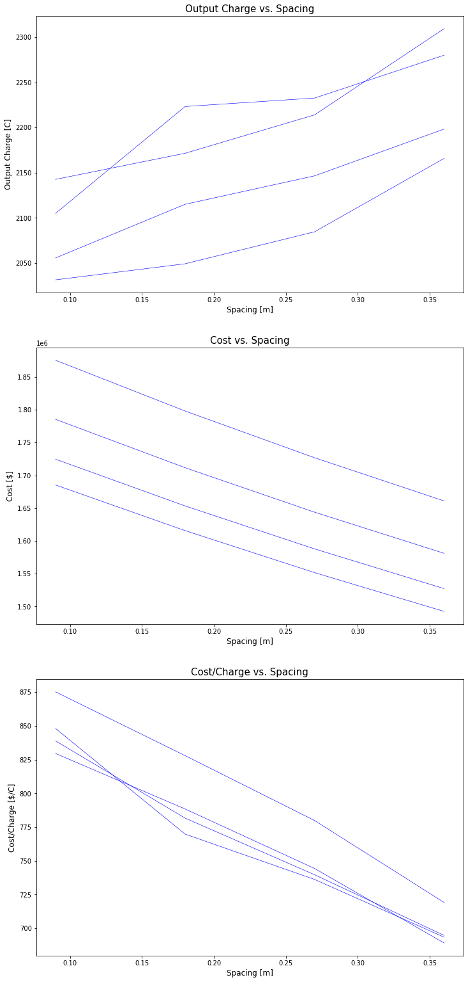
\includegraphics[width=3in]{fig31.png}
    \end{center}
    \renewcommand{\baselinestretch}{1}
    \small\normalsize
    \begin{quote}
    \caption[Batch 3 Spacing Trends]{Batch 3 Spacing Trends} \label{fig: f31}
    \end{quote}
\end{figure}

Having determined the output for the most economic configuration, we also obtained a value for the maximum output 
possible for the physical space in a highway setting. This value was 12334.1 C for 1600 m. 
We will use the selected charge outputs for the economical configuration and maximum output configuration to 
determine if this design can sustain an electric vehicle in the long term. 

See Figures \ref{fig: f32} and \ref{fig: f33} below for a visual representation of the most economical output and the maximum output configurations 
over 20 m.

\begin{figure}
    \begin{center}
    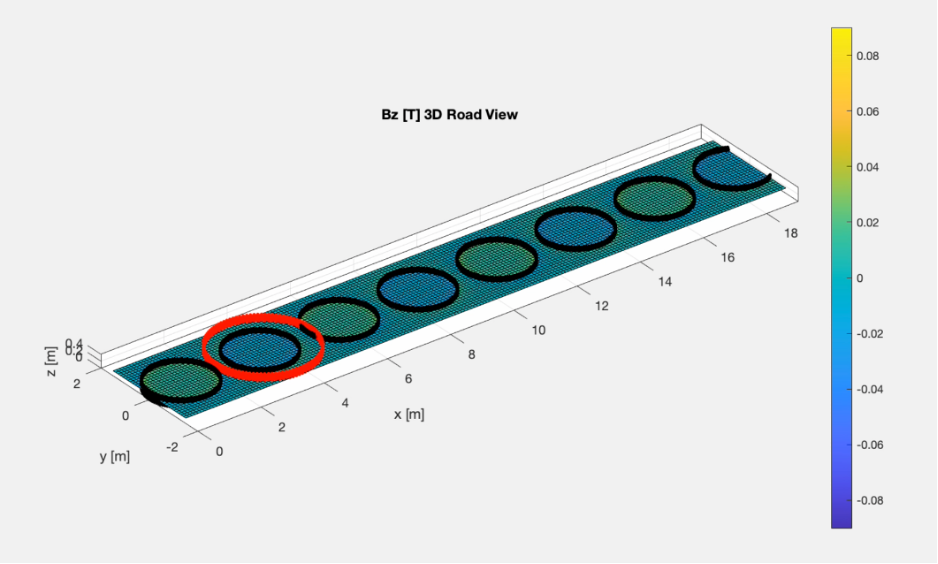
\includegraphics[width=5in]{fig32.png}
    \end{center}
    \renewcommand{\baselinestretch}{1}
    \small\normalsize
    \begin{quote}
    \caption[Economical Configuration Magnetic Field]{Economical Configuration Magnetic Field} \label{fig: f32}
    \end{quote}
\end{figure}

\begin{figure}
    \begin{center}
    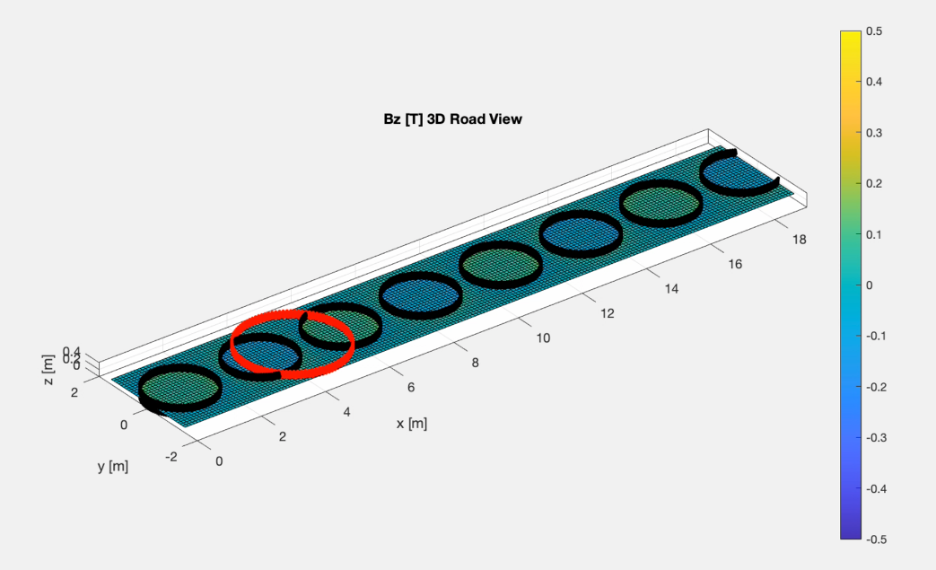
\includegraphics[width=5in]{fig33.png}
    \end{center}
    \renewcommand{\baselinestretch}{1}
    \small\normalsize
    \begin{quote}
    \caption[Maximum Output Configuration Magnetic Field]{Maximum Output Configuration Magnetic Field} \label{fig: f33}
    \end{quote}
\end{figure}

\section{Experimental Model}
Due to the circumstances surrounding COVID-19, results from in-person testing are delayed. For the purpose of 
this paper, the expected results will be discussed. As previously stated, the experimental model’s purpose 
is to provide a “real-world” comparison to the simulation results. Optimally, the data obtained through 
physical testing will validate the simulations and reinforce the variable relationships they produce.

The data from physical testing will be recorded using an oscilloscope which will yield voltage and current 
graphs pertaining to the receiving coil. The current graph will then be integrated with respect to time to 
obtain the cumulative charge acquired by the receiving coils. The modularity of the experimental model 
allows for variables such as transmitting coil current, spacing of the transmitting coils, height between 
the transmitting and receiving coils, and velocity of the receiving coil. The alteration of these variables 
will display their relationship with acquired charge. These relationships are then used to optimize the DWPT 
system to acquire the most charge. After multiple tests are run for the different variable scenarios, the 
testing team will plot the results and compare them with the plots produced by the simulations shown in 
Figures \ref{fig: f34} through \ref{fig: f37}.

\begin{figure}
    \begin{center}
    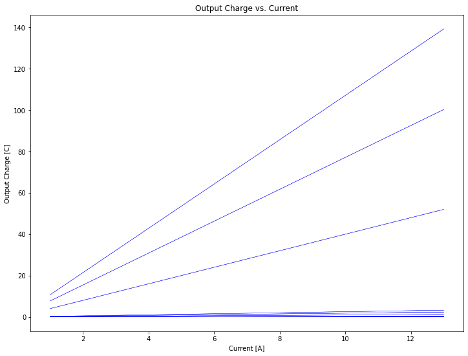
\includegraphics[width=3in]{fig34.png}
    \end{center}
    \renewcommand{\baselinestretch}{1}
    \small\normalsize
    \begin{quote}
    \caption[Experimental Model Expected Current Trend]{Experimental Model Expected Current Trend} \label{fig: f34}
    \end{quote}
\end{figure}

\begin{figure}
    \begin{center}
    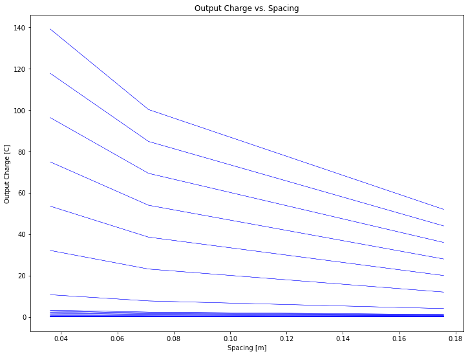
\includegraphics[width=3in]{fig35.png}
    \end{center}
    \renewcommand{\baselinestretch}{1}
    \small\normalsize
    \begin{quote}
    \caption[Experimental Model Expected Spacing Trend]{Experimental Model Expected Spacing Trend} \label{fig: f35}
    \end{quote}
\end{figure}

\begin{figure}
    \begin{center}
    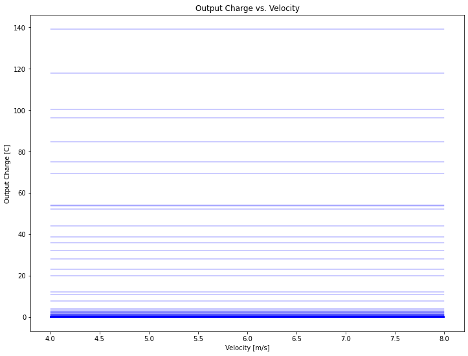
\includegraphics[width=3in]{fig36.png}
    \end{center}
    \renewcommand{\baselinestretch}{1}
    \small\normalsize
    \begin{quote}
    \caption[Experimental Model Expected Velocity Trend]{Experimental Model Expected Velocity Trend} \label{fig: f36}
    \end{quote}
\end{figure}

\begin{figure}
    \begin{center}
    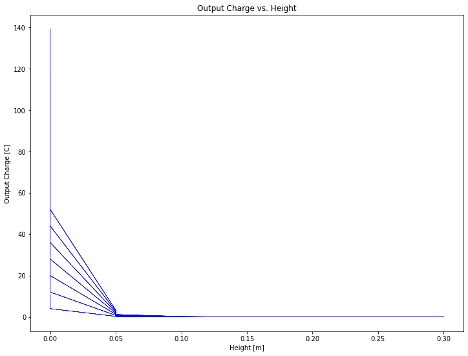
\includegraphics[width=3in]{fig37.png}
    \end{center}
    \renewcommand{\baselinestretch}{1}
    \small\normalsize
    \begin{quote}
    \caption[Experimental Model Expected Height Trend]{Experimental Model Expected Height Trend} \label{fig: f37}
    \end{quote}
\end{figure}

The comparison of the experimental model data and simulation data will reveal the accuracy of the current model. 
At first it is likely that the two data sets will deviate from each other due to unmodeled dynamics. 
The equations used to develop the model assume ideal conditions when that is not a likely scenario. 
After this, the iterative process of altering the model to better represent the experimental data begins. 
%Chapter 5

\renewcommand{\thechapter}{5}

\chapter{Discussion}

\section{Simulations}
To truly gauge the effectiveness of the simulated model, the results will be applied to two EVs: 
the Nissan Leaf and Tesla Model X. The Nissan Leaf is a budget EV with a 40 kilowatt-hour (kWh) 
battery \cite{noauthor_2021_nodate}. The Tesla Model X is a high-performing EV with a 100 kWh battery 
\cite{noauthor_model_nodate}. There will be two output configurations used from the simulation: the economic 
configuration and maximum output configuration. The economic configuration represents the most optimal 
combination of variables in terms of cost. The maximum output configuration represents the combination 
of variables which output the absolute most charge. See Section \ref{sec: s4.1.3} for the inputs of these 
configurations and how they were determined. 

Calculations and unit conversions are required to show the charge times of the elextric vehicles for each model. 
For the Nissan Leaf, the 40 kwh battery corresponds to 1.44 $\cdot$ 108 J. The Nissan Leaf battery is 360V 
\cite{noauthor_2021_nodate}. Using the formula 
\begin{equation}
    Energy \: [J] = Voltage \: [V] \cdot Coulombs \: [C]
\end{equation}
We determined the battery has 4.0 $\cdot$ 105 C. Using the output data, the distance covered by the vehicle 
is 1600 m (1 mile), and the speed is 30 m/s, so the time the simulated car takes is 53.33 s. In the economic 
configuration, the total charge was 2142.7 C, which corresponds to a charging rate of 40.2 C/s. In the maximum 
output configuration, the total charge is 12334.4 C, which corresponds to a charging rate of 231.3 C/s. 
The time it will take for the maximum output configuration to charge a Nissan Leaf battery is 
\begin{center}
    4.0 $\cdot$ 105 C/231.3 C/s = 1729.5 s = .484 hr
\end{center}
The time it will take for the economic model to charge a Nissan Leaf battery is 
\begin{center}
    4.0 $\cdot$ 105 C/40.2 C/s = 9955.7 s or 2.77 hr
\end{center}
The range of the Nissan Leaf is 149 miles (239792 m), and if the car is going at 30 m/sec, then the battery will 
run out of charge after 7993.07 s or 2.22 hr \cite{noauthor_2021_nodate}.

For the Tesla Model X, the 100 kwh, 350 V battery converts to 3.6 $\cdot$ 108 J \cite{noauthor_model_nodate}. The battery has 
1.0286 $\cdot$ 106 C. The time it will take for the maximum model to charge a Tesla Model X battery is 
\begin{center}
    1.0286 $\cdot$ 106 C/231.3 C/s = 4447.3 s or 1.24 hr
\end{center}
The time it will take for the economic model to charge a Tesla Model X battery is
\begin{center}
    1.0286 $\cdot$ 106 C/40.2 C/s = 25601.1 sec or 7.11 hr
\end{center}
The range of the Tesla Model X is 362 miles (578880 m), and if the car is going at 30 m/sec, then the battery 
will run out of charge after 19296 s or 5.36 hr \cite{noauthor_model_nodate}. See Table \ref{t11} for a summary of charging times.

\begin{table}[H]
    \caption[Charge Time Summary]{Charge Time Summary}
    \begin{center}
    \begin{tabular}{| p{0.5\textwidth} | p{0.2\textwidth} | p{0.2\textwidth} |}
    \hline
    Time [hr] & Nissan Leaf & Tesla Model X \\
    \hline \hline
    Battery life without DWPT & 2.22 & 5.36 \\
    \hline
    Charge with Economic Model & 2.77 & 7.11 \\
    \hline
    Charge with Maximum Output Model & .484 & 1.24 \\
    \hline
    \end{tabular}
    \end{center}
    \label{t11}
\end{table}

Using the data values from Table \ref{t11}, the distance it takes to fully charge the Nissan Leaf and Tesla Model X 
can be found. The distance it will take for the economic model to fully charge a Nissan Leaf is
\begin{center}
    972 sec $\cdot$ 30 m/s = 299160 m or 185.89 miles
\end{center}
The distance it will take for the maximum output model to fully charge a Nissan Leaf is
\begin{center}
    1742.4 sec $\cdot$ 30 m/s = 52272 m or 32.48 miles
\end{center}
The distance it will take for the economic model to fully charge a Tesla Model X is
\begin{center}
    25596 sec $\cdot$ 30 m/s = 767880 m or 477.14 miles
\end{center}
The distance it will take for the  maximum output model to fully charge a Tesla Model X is
\begin{center}
    4464 sec $\cdot$ 30 m/s = 133920 m or 83.21 miles.
\end{center}
See Table \ref{t12} for a summary of the charging distances.

\begin{table}[H]
    \caption[Charge Distance Summary]{Charge Distance Summary}
    \begin{center}
    \begin{tabular}{| p{0.5\textwidth} | p{0.2\textwidth} | p{0.2\textwidth} |}
    \hline
    Distance [miles] & Nissan Leaf & Tesla Model X \\
    \hline \hline
    Battery distance without DWPT & 149 & 360 \\
    \hline
    Charge with Economic Model & 185.89 & 477.14 \\
    \hline
    Charge with Maximum Output Model & 32.48 & 83.21 \\
    \hline
    \end{tabular}
    \end{center}
    \label{t12}
\end{table}

The maximum output model charges both the Nissan Leaf and the Tesla Model X faster than its battery depletes, 
so if this configuration were used, cars could use the chagrining lane only when needed and any other lanes at 
other times.  This could be beneficial because cars don’t need to be taking up space in the lane at all times.  
For the economic model, the charging rate is not enough to allow the vehicle to travel for infinite time. 
For the Nissan Leaf the economic model extends the battery life to about 11.2 hr and for the Tesla Model X it 
extends it to about 21.8 hr. Further, the maximum model can charge a budget EV very quickly. Although this model 
is not cost-efficient, the economic model still charges a budget EV at a fast enough rate to increase the range 
of the EV. Even higher performing EVs like the Tesla Model X will benefit greatly from both the economic and 
maximum models. The economic model provides enough power to extend both a budget and high-end electric vehicle’s 
battery length so that it is long enough for most trips. The new battery life is longer than recommended driving 
time for a single driver, so only trips with multiple drivers remain impacted by the range electric vehicles. 

\section{Experimental Model}
From the experiments, observations are expected to more or less confirm the results from simulation testing. 
Ideally, the relationships discovered from simulations would appear in the experimental model data as well. 
Furthermore, the experimental model allows for relatively quick but extensive data observation, which provides 
insight on how to improve simulations as well. In other words, the experimental model aids with an iterative process 
towards understanding the relationships relevant to wireless power transfer. Because the simulations provide a 
theoretical output for charge, test cases are necessary to determine the efficiency of DWPT in real life. 
Ultimately, the data and values collected from the experimental model would be crucial in proving the feasibility 
of wireless power transfer.

\section{Comparison to Existing Research}
The primary goal of our research has been to contribute to the growing body of knowledge dedicated to improving 
the efficiency and convenience of EVs. The Society of Automotive Engineering (SAE) J2954 standard is one notable 
recent advancement in this field. This standard sets industry-wide specifications for the interoperability of 
stationary wireless power transfer (WPT) systems in light-duty EVs. Our research can contribute to the expansion 
of these standards in the near future. There are two major differences between SAE J2954 and the scope of our research. 
First, SAE J2954 sets standards for stationary WPT while our research focused on dynamic WPT. 
Second, the WPT systems described in SAE J2954 utilize AC power while we tested a system using DC power. 
As mentioned in Section \ref{sec: s4.1}, we used some of the standards from SAE J2954 to define ranges of values of 
the variables tested in our simulations. We found that the values that resulted in the largest possible simulated 
charge output coincided with the standards set by the SAE, which validates our results. 

When running our simulations, we made assumptions that simplified the calculations due to constraints discussed 
in the following section. One of those assumptions was that the coils used in the DWPT system were perfectly 
wound circular coils of a constant radius. The simulations were also run assuming perfect alignment between the 
transmitting and receiving coils. In an analysis conducted by members of the Institute of Electrical and 
Electronics Engineers (IEEE), it was determined that solenoid coils were “smaller, lighter, [and] more tolerant of 
misalignment in a middle and large air gap” than circular coils \cite{fujita_dynamic_2017}. As mentioned briefly in 
Section \ref{sec: s4.1} and in the following section, the simulation and testing of different types of 
coils is one possible continuation of our research.
%Chapter 6

\renewcommand{\thechapter}{6}

\chapter{Future Directions}
\section{Simulations}
With more time and resources, the scope of our research can be expanded to mitigate the limitations highlighted in 
previous sections. Due to time constraints, a limited number of simulations were run that produced graphs showing 
only general trends with some error. The simulations were also run assuming ideal conditions. While this was 
sufficient to answer our research questions, more accurate results are needed if this system is to be physically 
implemented in the future. We first recommend that the numerical simulation be run with a step of .02 m or smaller 
between calculations to reduce error to a negligible value. The next recommendation would be to simulate real world 
conditions. This would include running simulations considering the real permeability of the space between the 
transmitting and receiving coils. For the purposes of our research, the simulation only considered perfect coils 
with a single radius. In the future, the simulation could be adapted to map different types of coils, such as pancake 
coils, to determine which configuration produces the greatest amount of power transfer. The simulation could also be 
adapted to determine how x- and y-components of the magnetic field contribute to the flux, and to determine the true 
efficiency of this power transfer system. A final recommendation for the improvement of the simulation would be to 
simulate imperfect alignment to determine whether that has significant effects on the charge output. If perfect 
alignment is required for maximum power output, another future step could be to incorporate this requirement in 
autonomous function.

\section{Experimental Model}
The purpose of the experimental model built as part of our research was to verify the results of the simulation. 
Due to material and space constraints, the test coils were arranged on a circular track. This does not accurately 
represent the alignment of coils on a straight track (i.e., a highway). The assumption was made that this model 
would scale to real world conditions, although this was not verified. Future endeavors could include improving the 
experimental model by creating a scale model of a standard highway and using materials that more accurately reflect 
real world conditions (such as concrete). The experimental model could also be improved by allowing for different 
types of coils to be tested, much like what was recommended for the simulation. The scope of the experimental model 
could also be expanded in the future to determine the effects of weather.
%Chapter 7

\renewcommand{\thechapter}{7}

\chapter{Conclusion}
In conclusion, the results of this project will add valuable knowledge to the field of wireless power transfer 
by creating a mathematical model to predict power output of a DWPT system based on specific variables. 
Physics predicts that DWPT infrastructure modeled like that in our simulation would be able to transfer enough 
power to increase the range of electric vehicles significantly. Furthermore, the project will demonstrate the 
accuracy of the model by applying it to a real-world small-scale experimental model.  If successful, this model 
can be used in the design of a DWPT system to be implemented in existing highways after more testing. This project 
has also shown that a valuable charging rate could be established for 875 \$/C.  This is only a relative cost, 
so further research should be done into cost models of these systems. 

There are multiple extensions of our project that can be pursued by other research teams building upon the 
limitations discussed here. Our project sought to simulate the use of a dynamic wireless charging system in o
rder to recommend optimal operating conditions and to generate a preliminary cost analysis. Future projects could 
include a policy recommendation report based on the findings of our research, which would discuss feasibility and 
cost of implementation in depth. There could be another project solely dedicated to modifying our simulation to 
better reflect real world conditions, taking changes in weather and material properties into consideration. We 
would also recommend a project focused on improving our physical experimental model and comparing any data collected 
to the results of the simulation discussed in this thesis. Our research is just one step in working towards 
encouraging the adoption of electric vehicles and reducing harmful vehicle emissions. There are many more avenues 
to be taken in continuing to build the gas station of the future.
\titleformat{\chapter}
{\normalfont\large}{Appendix \thechapter: }{1em}{}
%Appendix -- January 2015
\appendix
\renewcommand{\thechapter}{A}
\renewcommand{\chaptername}{Appendix}

\chapter{Equity Impact Report}

The Oxford English Dictionary defines equity as “the quality of being fair and impartial.” 
The phrase “equitable research” implies that a study is being carried out in such a way that 
its results are inclusive, causing little to no harm to any one community. 
Team FORMULA is committed to benign and beneficial involvement in research. 
The purpose of this report is to examine the unintended consequences of our research so 
that we may formulate an equitable recommendation as to the use of our results.

The results of our research could be used in the future implementation of wire- less charging lanes. 
There are many factors to be considered for this infrastructure, such as installation costs, location, 
and revenue scheme. State and federal gas taxes typically fund highway expansion and maintenance. 
An increase in the use of elec- tric vehicles, encouraged by new charging infrastructure, could 
cause a decrease in the already dwindling revenue collected through these taxes. To mitigate this lost revenue, 
tolls could be applied to wireless charging lanes. A survey conducted by CarMax and CleanTechnica found 
that 70\% of hybrid and electric vehicle owners had an annual income of \$75,000 or more 
\cite{noauthor_2017_nodate}. The assumption can be made that those who drive electric vehicles can 
afford to pay a toll to use charging lanes, which would benefit highway infrastructure as a whole. 

The people who are directly impacted by the results of our research are electric vehicle owners. 
They are the ones who will see quantifiable benefits in time saved on charging and increased driving range. 
Wireless changing lanes would also benefit poor communities and communities of color. 
The “Drive Change Drive Electric” campaign conducted a survey in which 83\% of respondents cited lack of 
charging stations as a barrier to electric vehicle adoption \cite{nhede_new_2019}. 
A wireless charging lane would encourage drivers to switch to electric vehicles by making charging more 
convenient, decreasing the demand for fossil fuels. Multiple studies have found that the costs of the fossil 
fuel industry “disproportionately fall upon people of color and low-income communities" \cite{noauthor_i-1631_nodate}.
A study published in Ap- plied Geography found that poor communities in Pennsylvania, West Virginia, and Ohio are 
“unequally exposed to pollution from unconventional gas wells" \cite{ogneva-himmelberger_spatial_2015}.
This is one way in which the scope of our research positively impacts a community outside of our intended audience.

Our research can be described as both equity neutral and equity positive. In the areas in which our results may 
have an adverse impact, we have proposed solutions in order to lessen the effects. We have also identified 
communities that we are unintentionally impacting and have determined that the effects of our research are 
beneficial to these communities.
%Appendix -- January 2015
\appendix
\renewcommand{\thechapter}{B}
\renewcommand{\chaptername}{Appendix}

\chapter{Code}
\label{sec: appB}

Code can be found stored at \\
https://github.com/katherinekemp/TeamFORMULA.git.

\renewcommand{\baselinestretch}{1}
\small\normalsize

\addcontentsline{toc}{chapter}{Glossary}
%List of Abbreviations


\renewcommand{\baselinestretch}{1}
\small\normalsize
\hbox{\ }

\vspace{.5in}

\begin{center}
\large{Glossary}
\end{center} 

\vspace{3pt}

\begin{supertabular}{p{0.2\textwidth}p{0.7\textwidth}}
AC/DC & Alternating current: oscillating current at a certain frequency; Direct current: continuous current with no oscillation \\
Ampere & SI unit of electric current \\
Coulomb & SI unit of electric charge \\
Current & Flow of electric charge \\
Diode & A circuit element with two terminals that only allows current to flow in one direction \\
Dynamic charging & The act of achieving power transfer to a battery by means of movement between a transmitting and receiving coil \\
Dynamic wireless power transfer (DWPT) & WPT of a moving entity, such as an EV \\
Electrical potential & The potential energy of an electrical charge \\
Electrical resistance & Opposition to the flow of electric charge \\
Electromagnetic Field & The physical field resulting from the change in velocity of a moving charged particle \\
Electromagnetic induction & The production of an electromagnetic field through a conductor via a changing magnetic field \\
Electromotive force (EMF) & A difference in electrical potential \\
Evanescent field & Oscillating electric or magnetic field that does not spread as an electromagnetic wave, and has no net energy flow in that region \\
Galvanometer & An instrument used to measure electrical current \\
Joule & SI unit of work (energy), 1 J = 1 N×m \\
Magnetic field & The area around a magnetic material or a moving electrical charge that exerts a force on a moving electrical charge \\
Magnetic flux & A measure of the flow of a magnetic field through a given area \\
Natural oscillation frequency & The frequency at which a circuit will oscillate in the absence of a driving or damping force \\
Power & Rate at which electrical energy is transferred per unit time \\
Range anxiety & Worry on the part of a person driving an electric car that the battery will run out of power before the destination or a suitable charging point is reached \\
Rectifier & An electrical device that converts alternating current to direct current via diodes \\
Resonance frequency & A frequency equal to or close to the natural oscillation frequency of a circuit \\
Resonators & Device that exhibits resonance or resonant behavior \\
Single-phase full-wave rectifier & A rectifier that is able to convert both the positive and negative parts of an alternating current into direct current \\
Single-phase half-wave rectifier & A rectifier that is only able to convert the positive part of an alternating current into direct current \\
Skin effect & The tendency of a high-frequency alternating current to flow through only the outer layer of a conductor \\
Solenoid & A coil of wire that acts as a magnet due to a current passing through it \\
Voltage & Electromotive force in terms of volts \\
Wireless Power Transfer (WPT) & A method of charging that does not require a wired connection between the power source and the electrical device in need of a charge \\
%$\alpha$ & alpha \\
%$\beta$  & beta \\
%&  \\ 
%IREAP & Institute for Research in Electronics and Applied Physics \\
%NSA & National Security Agency
\end{supertabular}


\addcontentsline{toc}{chapter}{Bibliography}
%\begin{thebibliography}{99}
\setlength{\parskip}{1em}

\bibitem{Agrawal1} G.P. Agrawal, {\em Nonlinear Fiber Optics} (Academic
Press, San Diego, CA, 2001), Chap. 1.
\bibitem{“2017 Hybrid/EV Survey Results.”} CarMax (2017), CarMax, www.carmax.com/articles/hybrid-electric-2017-survey-results
\bibitem{“2021 Nissan LEAF Range, Charging & Battery.”} (n.d.). Retrieved March 20, 2021, from https://www.nissanusa.com/vehicles/electric-cars/leaf/features/range-charging-battery.html
\bibitem{Arendash}, G. W., Sanchez-Ramos, J., Mori, T., Mamcarz, M., Lin, X., Runfeldt, M., … Cao, C. (2010). Electromagnetic Field Treatment Protects Against and Reverses Cognitive Impairment in Alzheimer’s Disease Mice. Journal of Alzheimer’s Disease, 19(1), 191–210. https://doi.org/10.3233/JAD-2010-1228
\bibitem{Arribas-Ibar} M, Nylund PA, Brem A. The Risk of Dissolution of Sustainable Innovation Ecosystems in Times of Crisis: The Electric Vehicle during the COVID-19 Pandemic. Sustainability. 2021; 13(3):1319. https://doi.org/10.3390/su13031319
\bibitem{Banerjee}, Debolina, et al. (2018) “I-1631 Takes Aim at the True Cost of Fossil Fuel Use for Communities of Color.” Puget Sound Sage, www.pugetsoundsage.org/true-cost-of-fossil-fuel-use-for-communities-of-color/
%\bibitem{Chen}, Z., Xu, C., Ma, C., Ren, W., & Cheng, H.-M. (2013). Lightweight and Flexible Graphene Foam Composites for High-Performance Electromagnetic Interference Shielding. Advanced Materials, 25(9), 1296–1300. https://doi.org/10.1002/adma.201204196
%\bibitem{Clement-Nyns}, K., Haesen, E., & Driesen, J. (2010). The Impact of Charging Plug-In Hybrid Electric Vehicles on a Residential Distribution Grid. IEEE Transactions on Power Systems, 25(1), 371–380.
%\bibitem{Eberhard}, M., & Tarpenning, M. (2018). The 21 st Century Electric Car Tesla Motors.
%\bibitem{Fisher}, T. M., Farley, K. B., Gao, Y., Bai, H., & Tse, Z. T. H. (2014). Electric vehicle wireless charging technology: a state-of-the-art review of magnetic coupling systems. Wireless Power Transfer, 1(02), 87–96. https://doi.org/10.1017/wpt.2014.8
\bibitem{Fujita}, T., Yasuda, T. and Akagi, H. (2017, July-August). A Dynamic Wireless Power Transfer System Applicable to a Stationary System. IEEE Transactions on Industry Applications, vol. 53, no. 4, pp. 3748-3757, doi: 10.1109/TIA.2017.2680400.
%\bibitem{Helmers}, E., & Marx, P. (2012). Electric cars: Technical characteristics and environmental impacts. Environmental Sciences Europe, 24(1). doi:10.1186/2190-4715-24-14
\bibitem{Houglum}, M. (2015). Oauth2client. https://github.com/googleapis/oauth2client 
%\bibitem{Ho}, S. L., Wang, J., Fu, W. N., & Sun, M. (2011). A Comparative Study Between Novel Witricity and Traditional Inductive Magnetic Coupling in Wireless Charging. IEEE Transactions on Magnetics, 47(5), 1522–1525. https://doi.org/10.1109/TMAG.2010.2091495
%\bibitem{Hunter}, J. D. (2007), Matplotlib: A 2D graphics environment, In 2007 Computing in Science & Engineering (pp. 90-95).
\bibitem{Joselow}, Maxine (2021) “Gasoline Car Sales to End by 2035 in Massachusetts” Scientific American. 
%\bibitem{J2954}: Wireless Power Transfer for Light-Duty Plug-in/Electric Vehicles and Alignment Methodology - SAE International. (n.d.). Retrieved April 1, 2021, from https://www.sae.org/standards/content/j2954_202010/
%\bibitem{Karam Hwang}, Jaeyong Cho, Dongwook Kim, Jaehyoung Park, Jong Hwa Kwon, Sang Il Kwak, … Seungyoung Ahn. (2017). An Autonomous Coil Alignment System for the DynamicWireless Charging of Electric Vehicles to Minimize Lateral Misalignment. Energies (19961073), 10(3), 1–20. https://doi.org/10.3390/en10030315
%\bibitem{Kostoff}, R. N., & Lau, C. G. Y. (2013). Combined biological and health effects of electromagnetic fields and other agents in the published literature. Technological Forecasting and Social Change, 80(7), 1331–1349. https://doi.org/10.1016/j.techfore.2012.12.006
\bibitem{Li, Y., Wang, W., Xing, L., Fan, Q., & Wang, H. (2018). Longitudinal safety evaluation of electric vehicles with the partial wireless charging lane on freeways. Accident Analysis & Prevention, 111, 133–141. https://doi.org/10.1016/j.aap.2017.11.036
\bibitem{Lu}, X., Wang, P., Niyato, D., Kim, D. I., & Han, Z. (2016). Wireless Charging Technologies: Fundamentals, Standards, and Network Applications. IEEE Communications Surveys & Tutorials, 18(2), 1413–1452. https://doi.org/10.1109/COMST.2015.2499783
\bibitem{Lukic}, S., & Pantic, Z. (2013). Cutting the Cord: Static and Dynamic Inductive Wireless Charging of Electric Vehicles. IEEE Electrification Magazine, 1(1), 57–64. https://doi.org/10.1109/MELE.2013.2273228
\bibitem{Lumpkins}, W. (2014). Nikola Tesla’s Dream Realized: Wireless power energy harvesting. IEEE Consumer Electronics Magazine, 3(1), 39–42. https://doi.org/10.1109/MCE.2013.2284940
\bibitem{Model x.} (n.d.). Retrieved April 02, 2021, from https://www.tesla.com/modelx
\bibitem{Mufson}, Steven “General Motors to eliminate gasoline and diesel light-duty cars and SUVs by 2035” The Washington Post. 28 Jan 2021.
\bibitem{Nabel}, R pydrive (2016) Retrieved March 30, 2021 from
https://pypi.org/project/PyDrive/ 
\bibitem{Nhede}, Nicholas (2020). “New Study Reveals Interesting Statistics on EV Ownership and Consumer Interest.” Smart Energy International, 16 Jan. 2020, www.smart-energy.com/industry-sectors/smart-energy/new-study-reveals-interesting-statistics-on-ev-ownership-and-consumer-interest/
\bibitem{Ogneva-Himmelberger}, Yelena, and Liyao Huang (2015). “Spatial Distribution of Unconventional Gas Wells and Human Populations in the Marcellus Shale in the United States: Vulnerability Analysis.” Applied Geography, vol. 60, June 2015, pp. 165–174., doi:10.1016/j.apgeog.2015.03.011.
\bibitem{Onar}, O. C., Miller, J. M., Campbell, S. L., Coomer, C., White, C. P., & Seiber, L. E. (2013). A novel wireless power transfer for in-motion EV/PHEV charging. In 2013 Twenty-Eighth Annual IEEE Applied Power Electronics Conference and Exposition (APEC) (pp. 3073–3080). Long Beach, CA, USA: IEEE. https://doi.org/10.1109/APEC.2013.6520738
\bibitem{Onat}, N. C., Noori, M., Kucukvar, M., Zhao, Y., Tatari, O., & Chester, M. (2017). Exploring the suitability of electric vehicles in the United States. Energy, 121, 631–642. https://doi.org/10.1016/j.energy.2017.01.035
\bibitem{Panchal}, C., Stegen, S., & Lu, J. (2018). Review of static and dynamic wireless electric vehicle charging system. Engineering Science and Technology, an International Journal, 21(5), 922–937. https://doi.org/10.1016/j.jestch.2018.06.015
\bibitem{Parmesh}, K., Neriya, R. P., & Kumar, M. V. (2017). Wireless Charging System for Electric Vehicles. International Journal of Vehicle Structures & Systems (IJVSS), 9(1), 23–26. https://doi.org/10.4273/ijvss.9.1.05
\bibitem{Pearre}, N. S., Kempton, W., Guensler, R. L., & Elango, V. V. (2011). Electric vehicles: How much range is required for a day’s driving? Transportation Research Part C: Emerging Technologies, 19(6), 1171–1184. https://doi.org/10.1016/j.trc.2010.12.010
\bibitem{Queval Loic} (2021). Biot Savart magnetic Toolbox (https://github.com/lqueval/BSmag), GitHub. Retrieved March 23, 2021.
\bibitem{Rakhymbay}, A., Khamitov, A., Bagheri, M., Alimkhanuly, B., Lu, M., Phung, T., … Phung, T. (2018). Precise Analysis on Mutual Inductance Variation in Dynamic Wireless Charging of Electric Vehicle. Energies, 11(3), 624. https://doi.org/10.3390/en11030624
\bibitem{Reback}, J., MacKinney, W., Jbrockmendal, Bossche, J.V.D., Augspurger, T., Cloud, P. (2021) pandas-dev/pandas: Pandas 1.2.3 (Version v1.2.3). Zenodo 
http://doi.org/10.5281/zenodo.4572994 
\bibitem{Resonant circuits} | Brilliant Math & Science Wiki. (n.d.). Retrieved December 11, 2018, from https://brilliant.org/wiki/resonant-circuits/
\bibitem{Skvarenina}, T. L. (2001). The Power Electronics Handbook. CRC Press.
\bibitem{Throngnumchai}, K., Hanamura, A., Naruse, Y., & Takeda, K. (2013). Design and evaluation of a wireless power transfer system with road embedded transmitter coils for dynamic charging of electric vehicles. In 2013 World Electric Vehicle Symposium and Exhibition (EVS27) (pp. 1–10). https://doi.org/10.1109/EVS.2013.6914937
\bibitem{Tiikkaja}, M., Aro, A. L., Alanko, T., Lindholm, H., Sistonen, H., Hartikainen, J. E. K., … Hietanen, M. (2013). Electromagnetic interference with cardiac pacemakers and implantable cardioverter-defibrillators from low-frequency electromagnetic fields in vivo. EP Europace, 15(3), 388–394. https://doi.org/10.1093/europace/eus345
\bibitem{US EPA, OA.} (2015). Sources of Greenhouse Gas Emissions [Overviews and Factsheets]. Retrieved October 1, 2018, from https://www.epa.gov/ghgemissions/sources-greenhouse-gas-emissions
\bibitem{US EPA, OAR.} (2016). Greenhouse Gas Emissions from a Typical Passenger Vehicle [Overviews and Factsheets]. Retrieved October 1, 2018, from https://www.epa.gov/greenvehicles/greenhouse-gas-emissions-typical-passenger-vehicle
\bibitem{Vilas}, M. google (2016) Retrieved March 30, 2021 from https://breakingcode.wordpress.com/
\bibitem{What is magnetic flux?} (n.d.). Retrieved October 1, 2018, from https://www.khanacademy.org/science/physics/magnetic-forces-and-magnetic-fields/magnetic-flux-faradays-law/a/what-is-magnetic-flux
\bibitem{Xiang}, L., Sun, Y., Tang, C., Dai, X., & Jiang, C. (2017). Design of crossed DD coil for dynamic wireless charging of electric vehicles. In 2017 IEEE PELS Workshop on Emerging Technologies: Wireless Power Transfer (WoW) (pp. 1–5). https://doi.org/10.1109/WoW.2017.7959422
\bibitem{Young}, H. D., & Freedman, R. A. (2016). University Physics with Modern Physics (14th ed.). Pearson.
\end{thebibliography}
 %Delete this line if using Bibtex or Natbib
\bibliographystyle{unsrt}
\newpage
\bibliography{formula}

\end{document}
